% Options for packages loaded elsewhere
%DIF LATEXDIFF DIFFERENCE FILE
%DIF DEL paper-v1.tex   Mon Mar 25 10:53:38 2024
%DIF ADD paper.tex      Mon Mar 25 20:02:06 2024
\PassOptionsToPackage{unicode}{hyperref}
\PassOptionsToPackage{hyphens}{url}
\PassOptionsToPackage{dvipsnames,svgnames,x11names}{xcolor}
%
\documentclass[
  super,
  preprint,
  3p]{elsarticle}

\usepackage{amsmath,amssymb}
\usepackage{setspace}
\usepackage{iftex}
\ifPDFTeX
  \usepackage[T1]{fontenc}
  \usepackage[utf8]{inputenc}
  \usepackage{textcomp} % provide euro and other symbols
\else % if luatex or xetex
  \usepackage{unicode-math}
  \defaultfontfeatures{Scale=MatchLowercase}
  \defaultfontfeatures[\rmfamily]{Ligatures=TeX,Scale=1}
\fi
\usepackage{lmodern}
\ifPDFTeX\else  
    % xetex/luatex font selection
\fi
% Use upquote if available, for straight quotes in verbatim environments
\IfFileExists{upquote.sty}{\usepackage{upquote}}{}
\IfFileExists{microtype.sty}{% use microtype if available
  \usepackage[]{microtype}
  \UseMicrotypeSet[protrusion]{basicmath} % disable protrusion for tt fonts
}{}
\makeatletter
\@ifundefined{KOMAClassName}{% if non-KOMA class
  \IfFileExists{parskip.sty}{%
    \usepackage{parskip}
  }{% else
    \setlength{\parindent}{0pt}
    \setlength{\parskip}{6pt plus 2pt minus 1pt}}
}{% if KOMA class
  \KOMAoptions{parskip=half}}
\makeatother
\usepackage{xcolor}
\setlength{\emergencystretch}{3em} % prevent overfull lines
\setcounter{secnumdepth}{5}
% Make \paragraph and \subparagraph free-standing
\ifx\paragraph\undefined\else
  \let\oldparagraph\paragraph
  \renewcommand{\paragraph}[1]{\oldparagraph{#1}\mbox{}}
\fi
\ifx\subparagraph\undefined\else
  \let\oldsubparagraph\subparagraph
  \renewcommand{\subparagraph}[1]{\oldsubparagraph{#1}\mbox{}}
\fi


\providecommand{\tightlist}{%
  \setlength{\itemsep}{0pt}\setlength{\parskip}{0pt}}\usepackage{longtable,booktabs,array}
\usepackage{calc} % for calculating minipage widths
% Correct order of tables after \paragraph or \subparagraph
\usepackage{etoolbox}
\makeatletter
\patchcmd\longtable{\par}{\if@noskipsec\mbox{}\fi\par}{}{}
\makeatother
% Allow footnotes in longtable head/foot
\IfFileExists{footnotehyper.sty}{\usepackage{footnotehyper}}{\usepackage{footnote}}
\makesavenoteenv{longtable}
\usepackage{graphicx}
\makeatletter
\def\maxwidth{\ifdim\Gin@nat@width>\linewidth\linewidth\else\Gin@nat@width\fi}
\def\maxheight{\ifdim\Gin@nat@height>\textheight\textheight\else\Gin@nat@height\fi}
\makeatother
% Scale images if necessary, so that they will not overflow the page
% margins by default, and it is still possible to overwrite the defaults
% using explicit options in \includegraphics[width, height, ...]{}
\setkeys{Gin}{width=\maxwidth,height=\maxheight,keepaspectratio}
% Set default figure placement to htbp
\makeatletter
\def\fps@figure{htbp}
\makeatother

%DIF 82a82-95
\usepackage{booktabs} %DIF > 
\usepackage{longtable} %DIF > 
\usepackage{array} %DIF > 
\usepackage{multirow} %DIF > 
\usepackage{wrapfig} %DIF > 
\usepackage{float} %DIF > 
\usepackage{colortbl} %DIF > 
\usepackage{pdflscape} %DIF > 
\usepackage{tabu} %DIF > 
\usepackage{threeparttable} %DIF > 
\usepackage{threeparttablex} %DIF > 
\usepackage[normalem]{ulem} %DIF > 
\usepackage{makecell} %DIF > 
\usepackage{xcolor} %DIF > 
%DIF -------
\makeatletter
\@ifpackageloaded{caption}{}{\usepackage{caption}}
\AtBeginDocument{%
\ifdefined\contentsname
  \renewcommand*\contentsname{Table of contents}
\else
  \newcommand\contentsname{Table of contents}
\fi
\ifdefined\listfigurename
  \renewcommand*\listfigurename{List of Figures}
\else
  \newcommand\listfigurename{List of Figures}
\fi
\ifdefined\listtablename
  \renewcommand*\listtablename{List of Tables}
\else
  \newcommand\listtablename{List of Tables}
\fi
\ifdefined\figurename
  \renewcommand*\figurename{Figure}
\else
  \newcommand\figurename{Figure}
\fi
\ifdefined\tablename
  \renewcommand*\tablename{Table}
\else
  \newcommand\tablename{Table}
\fi
}
\@ifpackageloaded{float}{}{\usepackage{float}}
\floatstyle{ruled}
\@ifundefined{c@chapter}{\newfloat{codelisting}{h}{lop}}{\newfloat{codelisting}{h}{lop}[chapter]}
\floatname{codelisting}{Listing}
\newcommand*\listoflistings{\listof{codelisting}{List of Listings}}
\makeatother
\makeatletter
\makeatother
\makeatletter
\@ifpackageloaded{caption}{}{\usepackage{caption}}
\@ifpackageloaded{subcaption}{}{\usepackage{subcaption}}
\makeatother
\journal{European Transport Research Review}
\ifLuaTeX
  \usepackage{selnolig}  % disable illegal ligatures
\fi
\usepackage[]{natbib}
\bibliographystyle{elsarticle-num}
\usepackage{bookmark}

\IfFileExists{xurl.sty}{\usepackage{xurl}}{} % add URL line breaks if available
\urlstyle{same} % disable monospaced font for URLs
\hypersetup{
%DIF 134-135c148-149
%DIF <   pdftitle={CRUSE to Safe Cycling in Ireland},
%DIF <   pdfauthor={Robin Lovelace; Joey Talbot; Eugeni Vidal-Tortosa; Hussein Mahfouz; Elaine Brick; Peter Wright; Gary O'Tool; Dan Brennan; Suzanne Meade},
%DIF -------
  pdftitle={Cycle Route Uptake and Scenario Estimation (CRUSE): an approach for developing strategic cycle network planning tools}, %DIF > 
  pdfauthor={Robin Lovelace; Joey Talbot; Eugeni Vidal-Tortosa; Hussein Mahfouz; Elaine Brick; Peter Wright; Gary O'Toole; Dan Brennan; Suzanne Meade}, %DIF > 
%DIF -------
  pdfkeywords={Cycling, Open-source, Road Safety, Active Travel},
  colorlinks=true,
  linkcolor={blue},
  filecolor={Maroon},
  citecolor={Blue},
  urlcolor={Blue},
  pdfcreator={LaTeX via pandoc}}

\setlength{\parindent}{6pt}
%DIF PREAMBLE EXTENSION ADDED BY LATEXDIFF
%DIF UNDERLINE PREAMBLE %DIF PREAMBLE
\RequirePackage[normalem]{ulem} %DIF PREAMBLE
\RequirePackage{color}\definecolor{RED}{rgb}{1,0,0}\definecolor{BLUE}{rgb}{0,0,1} %DIF PREAMBLE
\providecommand{\DIFadd}[1]{{\protect\color{blue}\uwave{#1}}} %DIF PREAMBLE
\providecommand{\DIFdel}[1]{{\protect\color{red}\sout{#1}}}                      %DIF PREAMBLE
%DIF SAFE PREAMBLE %DIF PREAMBLE
\providecommand{\DIFaddbegin}{} %DIF PREAMBLE
\providecommand{\DIFaddend}{} %DIF PREAMBLE
\providecommand{\DIFdelbegin}{} %DIF PREAMBLE
\providecommand{\DIFdelend}{} %DIF PREAMBLE
\providecommand{\DIFmodbegin}{} %DIF PREAMBLE
\providecommand{\DIFmodend}{} %DIF PREAMBLE
%DIF FLOATSAFE PREAMBLE %DIF PREAMBLE
\providecommand{\DIFaddFL}[1]{\DIFadd{#1}} %DIF PREAMBLE
\providecommand{\DIFdelFL}[1]{\DIFdel{#1}} %DIF PREAMBLE
\providecommand{\DIFaddbeginFL}{} %DIF PREAMBLE
\providecommand{\DIFaddendFL}{} %DIF PREAMBLE
\providecommand{\DIFdelbeginFL}{} %DIF PREAMBLE
\providecommand{\DIFdelendFL}{} %DIF PREAMBLE
\newcommand{\DIFscaledelfig}{0.5}
%DIF HIGHLIGHTGRAPHICS PREAMBLE %DIF PREAMBLE
\RequirePackage{settobox} %DIF PREAMBLE
\RequirePackage{letltxmacro} %DIF PREAMBLE
\newsavebox{\DIFdelgraphicsbox} %DIF PREAMBLE
\newlength{\DIFdelgraphicswidth} %DIF PREAMBLE
\newlength{\DIFdelgraphicsheight} %DIF PREAMBLE
% store original definition of \includegraphics %DIF PREAMBLE
\LetLtxMacro{\DIFOincludegraphics}{\includegraphics} %DIF PREAMBLE
\newcommand{\DIFaddincludegraphics}[2][]{{\color{blue}\fbox{\DIFOincludegraphics[#1]{#2}}}} %DIF PREAMBLE
\newcommand{\DIFdelincludegraphics}[2][]{% %DIF PREAMBLE
\sbox{\DIFdelgraphicsbox}{\DIFOincludegraphics[#1]{#2}}% %DIF PREAMBLE
\settoboxwidth{\DIFdelgraphicswidth}{\DIFdelgraphicsbox} %DIF PREAMBLE
\settoboxtotalheight{\DIFdelgraphicsheight}{\DIFdelgraphicsbox} %DIF PREAMBLE
\scalebox{\DIFscaledelfig}{% %DIF PREAMBLE
\parbox[b]{\DIFdelgraphicswidth}{\usebox{\DIFdelgraphicsbox}\\[-\baselineskip] \rule{\DIFdelgraphicswidth}{0em}}\llap{\resizebox{\DIFdelgraphicswidth}{\DIFdelgraphicsheight}{% %DIF PREAMBLE
\setlength{\unitlength}{\DIFdelgraphicswidth}% %DIF PREAMBLE
\begin{picture}(1,1)% %DIF PREAMBLE
\thicklines\linethickness{2pt} %DIF PREAMBLE
{\color[rgb]{1,0,0}\put(0,0){\framebox(1,1){}}}% %DIF PREAMBLE
{\color[rgb]{1,0,0}\put(0,0){\line( 1,1){1}}}% %DIF PREAMBLE
{\color[rgb]{1,0,0}\put(0,1){\line(1,-1){1}}}% %DIF PREAMBLE
\end{picture}% %DIF PREAMBLE
}\hspace*{3pt}}} %DIF PREAMBLE
} %DIF PREAMBLE
\LetLtxMacro{\DIFOaddbegin}{\DIFaddbegin} %DIF PREAMBLE
\LetLtxMacro{\DIFOaddend}{\DIFaddend} %DIF PREAMBLE
\LetLtxMacro{\DIFOdelbegin}{\DIFdelbegin} %DIF PREAMBLE
\LetLtxMacro{\DIFOdelend}{\DIFdelend} %DIF PREAMBLE
\DeclareRobustCommand{\DIFaddbegin}{\DIFOaddbegin \let\includegraphics\DIFaddincludegraphics} %DIF PREAMBLE
\DeclareRobustCommand{\DIFaddend}{\DIFOaddend \let\includegraphics\DIFOincludegraphics} %DIF PREAMBLE
\DeclareRobustCommand{\DIFdelbegin}{\DIFOdelbegin \let\includegraphics\DIFdelincludegraphics} %DIF PREAMBLE
\DeclareRobustCommand{\DIFdelend}{\DIFOaddend \let\includegraphics\DIFOincludegraphics} %DIF PREAMBLE
\LetLtxMacro{\DIFOaddbeginFL}{\DIFaddbeginFL} %DIF PREAMBLE
\LetLtxMacro{\DIFOaddendFL}{\DIFaddendFL} %DIF PREAMBLE
\LetLtxMacro{\DIFOdelbeginFL}{\DIFdelbeginFL} %DIF PREAMBLE
\LetLtxMacro{\DIFOdelendFL}{\DIFdelendFL} %DIF PREAMBLE
\DeclareRobustCommand{\DIFaddbeginFL}{\DIFOaddbeginFL \let\includegraphics\DIFaddincludegraphics} %DIF PREAMBLE
\DeclareRobustCommand{\DIFaddendFL}{\DIFOaddendFL \let\includegraphics\DIFOincludegraphics} %DIF PREAMBLE
\DeclareRobustCommand{\DIFdelbeginFL}{\DIFOdelbeginFL \let\includegraphics\DIFdelincludegraphics} %DIF PREAMBLE
\DeclareRobustCommand{\DIFdelendFL}{\DIFOaddendFL \let\includegraphics\DIFOincludegraphics} %DIF PREAMBLE
%DIF LISTINGS PREAMBLE %DIF PREAMBLE
\RequirePackage{listings} %DIF PREAMBLE
\RequirePackage{color} %DIF PREAMBLE
\lstdefinelanguage{DIFcode}{ %DIF PREAMBLE
%DIF DIFCODE_UNDERLINE %DIF PREAMBLE
  moredelim=[il][\color{red}\sout]{\%DIF\ <\ }, %DIF PREAMBLE
  moredelim=[il][\color{blue}\uwave]{\%DIF\ >\ } %DIF PREAMBLE
} %DIF PREAMBLE
\lstdefinestyle{DIFverbatimstyle}{ %DIF PREAMBLE
	language=DIFcode, %DIF PREAMBLE
	basicstyle=\ttfamily, %DIF PREAMBLE
	columns=fullflexible, %DIF PREAMBLE
	keepspaces=true %DIF PREAMBLE
} %DIF PREAMBLE
\lstnewenvironment{DIFverbatim}{\lstset{style=DIFverbatimstyle}}{} %DIF PREAMBLE
\lstnewenvironment{DIFverbatim*}{\lstset{style=DIFverbatimstyle,showspaces=true}}{} %DIF PREAMBLE
%DIF END PREAMBLE EXTENSION ADDED BY LATEXDIFF

\begin{document}

\begin{frontmatter}
\title{\DIFaddbegin \DIFadd{Cycle Route Uptake and Scenario Estimation (}\DIFaddend CRUSE\DIFdelbegin \DIFdel{to Safe Cycling in Ireland }%DIFDELCMD < \\\large{An Open Source Tool to
%DIFDELCMD < Support Active Travel} %%%
\DIFdelend \DIFaddbegin \DIFadd{): an approach
for developing strategic cycle network planning tools}\DIFaddend }
\author[1]{Robin Lovelace%
\corref{cor1}%
}
 \ead{r.lovelace@leeds.ac.uk} 
\author[1]{Joey Talbot%
%
}

\author[1]{Eugeni Vidal-Tortosa%
%
}

\author[1]{Hussein Mahfouz%
%
}

\author[2]{Elaine Brick%
%
}

\author[3]{Peter Wright%
%
}

\author[2]{Gary O'\DIFdelbegin \DIFdel{Tool}\DIFdelend \DIFaddbegin \DIFadd{Toole}\DIFaddend %
%
}

\author[4]{Dan Brennan%
%
}

\author[4]{Suzanne Meade%
%
}


\affiliation[1]{organization={University of
Leeds},addressline={Institute for Transport Studies, Leeds, LS2 9JT,
United Kingdom},postcodesep={}}
\affiliation[2]{organization={AECOM},addressline={Unit 6, Galway
Technology Park, Parkmore, Galway, Ireland},postcodesep={}}
\affiliation[3]{organization={AECOM},addressline={Winslade House,
Winslade Park, Manor Drive, Clyst St Mary, Exeter, EX5 1FY,
UK},postcodesep={}}
\affiliation[4]{organization={Transport Infrastructure
Ireland},addressline={Parkgate Business Centre, Parkgate Street, Dublin
8, D08 DK10, Ireland},postcodesep={}}

\cortext[cor1]{Corresponding author}









        
\begin{abstract}
\DIFdelbegin \DIFdel{Legislation mandates improved road safety and decarbonisation of
predominantly road-based transport network in Ireland and other
countries. Increasing cycling transport, making it safer and more
attractive, is essential to this end. Cycling in Ireland represents only
3\% of total modal share as of the latest Census (2016), but accounts
for 20\% of serious injuries and 7\% of all fatalities. A planning tool
based on high resolution datasets on baseline and potential cycling
levels could greatly assist in achieving this goal.
}%DIFDELCMD < 

%DIFDELCMD < %%%
\DIFdelend This paper describes \DIFdelbegin \DIFdel{the design, features and potential use of }\DIFdelend \DIFaddbegin \DIFadd{an approach for developing strategic cycle network
planning tools. Based on our experience developing and deploying }\DIFaddend the
Cycle Route Uptake and Scenario Estimation (CRUSE) Tool for Ireland\DIFdelbegin \DIFdel{was
commissioned to support cycle network planning, safety interventions, business cases and project evaluation. The resulting web application is
available at }%DIFDELCMD < \url{https://cruse.bike/}%%%
\DIFdel{, enabling }\DIFdelend \DIFaddbegin \DIFadd{, we
outline the underlying methods, including disaggregation of
origin-destination data, incorporation of additional trip purposes,
routing, scenario generation, and development of an intuitive user
interface. Commissioned and used by Transport Infrastructure Ireland,
CRUSE provides estimates of current and potential future cycling levels
under `snapshot' scenarios to inform investment decisions. The publicly
available results at https://cruse.bike/ enable }\DIFaddend planners, engineers, and
other stakeholders to make more evidence-based decisions. CRUSE goes
beyond previous work \DIFdelbegin \DIFdel{in several important ways. It models }\DIFdelend \DIFaddbegin \DIFadd{by: modeling }\DIFaddend networks at high \DIFdelbegin \DIFdel{levels of geographic resolution, simulates a wide range of trips
including recreational, }\DIFdelend \DIFaddbegin \DIFadd{spatial resolution;
simulating multiple trip purposes (}\DIFaddend social, shopping\DIFdelbegin \DIFdel{and personal trips,
}\DIFdelend \DIFaddbegin \DIFadd{, personal utility,
recreational, and cycle touring) }\DIFaddend in addition to \DIFdelbegin \DIFdel{trips to work and primary, secondary and tertiary education
locations. The tool provides key `denominator' information to enable
reporting of collision rates per billion km cycled.
}%DIFDELCMD < 

%DIFDELCMD < %%%
\DIFdel{Another key feature of CRUSE is its use of frequently-updated
OpenStreetMap data for route calculation and ``cycle friendliness''
estimates of all links on the network.
CRUSE provides three network types : the }\DIFdelend \DIFaddbegin \DIFadd{using official
origin-destination data; and providing estimates of `quietness' (a proxy
for cyclist comfort and route preference) at the route segment level.
Three network types --- }\DIFaddend `Fastest'\DIFdelbegin \DIFdel{network highlights routes for directness;
`Quietest'prioritises cycle friendliness}\DIFdelend \DIFaddbegin \DIFadd{, `Balanced'}\DIFaddend , and `\DIFdelbegin \DIFdel{Balanced' represents a
balance between speed and comfort. Trips are generated based on origin
and
destination data from the 2016 Census in combination with modeled
demand data to estimate current and potential future cycling levels at
area, route, and network levels for each county in Ireland. }%DIFDELCMD < 

%DIFDELCMD < %%%
\DIFdel{For investment in cycling to deliver on the huge potential benefits, cycling must become safer. With growth in the
ebike market, CRUSE will
help inform inter-urban and rural networks to support the transfer of
trips to sustainable modes for longer journeys. Provision of open access
data in a publicly available web tool will address the challenges faced
by counties across Ireland in meeting their sustainability commitments.
The experience of developing a deploying CRUSE are relevant to countries
with sustainable transport policies worldwide}\DIFdelend \DIFaddbegin \DIFadd{Quietest' --- help
plan both arterial and residential cycle networks. Workshops and
unstructured interviews with stakeholders show that the tool is already
being used in practice to inform urban, inter-urban, and rural network
planning. The approach is flexible and open-source, allowing the
underlying ideas and code to be adapted, supporting effective cycling
policies and interventions internationally}\DIFaddend .
\end{abstract}





\begin{keyword}
    Cycling \sep Open-source \sep Road Safety \sep 
    Active Travel
\end{keyword}
\end{frontmatter}

\setstretch{2}
\newpage{}

\section{Introduction}\label{introduction}

\DIFdelbegin \DIFdel{High energy transport systems }\DIFdelend \DIFaddbegin \DIFadd{Transport systems dominated by heavy and powerful private cars are
inefficient, dangerous, and unhealthy. Cars }\DIFaddend are a major \DIFdelbegin \DIFdel{contributor to climate change
}\DIFdelend \DIFaddbegin \DIFadd{and growing
source of greenhouse gas emissions causing climate change
\mbox{%DIFAUXCMD
\citep{winkler2023}}\hspace{0pt}%DIFAUXCMD
}\DIFaddend , a leading cause of premature death and injury due
to road traffic collisions \DIFaddbegin \DIFadd{\mbox{%DIFAUXCMD
\citep{globals2018} }\hspace{0pt}%DIFAUXCMD
}\DIFaddend , and a cause of disease
due to \DIFdelbegin \DIFdel{airborne and noise pollutants.
Conversely, evidence-based and effective transport }\emph{\DIFdel{policies}} %DIFAUXCMD
\DIFdel{have
great potential to decarbonize economies, improve public health, and
save lives.
}%DIFDELCMD < 

%DIFDELCMD < %%%
\DIFdelend \DIFaddbegin \DIFadd{physical inactivity and air, noise and (from tyres) microplastic
pollution \mbox{%DIFAUXCMD
\citep{mattsson2023} }\hspace{0pt}%DIFAUXCMD
\mbox{%DIFAUXCMD
\citep{welch2023} }\hspace{0pt}%DIFAUXCMD
\mbox{%DIFAUXCMD
\citep{cavallaro2024}}\hspace{0pt}%DIFAUXCMD
.
}\DIFaddend Transport is responsible for 23\% of global greenhouse gas (GHG)
emissions, 70\% of which are from road transport\DIFdelbegin \DIFdel{. Nearly half of these
}\DIFdelend \DIFaddbegin \DIFadd{, with passenger cars
accounting for nearly half of transport }\DIFaddend emissions (around 10\% of global
emissions) \DIFdelbegin \DIFdel{are from passenger cars
}\DIFdelend \citep{jaramillo2022}. The transport system encourages,
enables and in some cases enforces unsustainable lifestyles. Services
that are only accessible by car lock-in car dependency
\citep{gray2001, shergold2012, motte-baumvol2010}.

\DIFdelbegin \DIFdel{Recognizing the growing evidence of such impacts of poorly designed and
performing transport
systems , }\DIFdelend \DIFaddbegin \DIFadd{Growing evidence of the negative impacts of car-dependent transport
systems has led }\DIFaddend governments in many countries \DIFdelbegin \DIFdel{have }\DIFdelend \DIFaddbegin \DIFadd{to }\DIFaddend set targets and \DIFdelbegin \DIFdel{taken }\DIFdelend \DIFaddbegin \DIFadd{take
}\DIFaddend actions. In the context of climate, road safety and physicial inactivity
crises, policies to improve transport systems can be classified
according to the `Avoid-Shift-Improve' (ASI) framework
\citep{jaramillo2022}. The ASI framework highlights the importance of
demand reduction (\emph{avoid}ing unnecessary trips), in addition to
mode \emph{shift} to sustainable modes and \emph{improvement} of
existing energy converters, in that order.

Building cycle networks represents a relatively `quick win' within the
context of decarbonization \citep{brand2020} and sustainable mobility
\citep{burns2013}. Although cycling uptake appears on the surface to
only relate to the `shift' part of the ASI framework, closer
consideration of the knock-on impacts of cycling uptake shows that it
can also help avoid unnecessary trips \citep{nello-deakin2020}.
Furthermore, highly efficient ebikes --- which are seeing rapid uptake
in Ireland and other countries --- outperform electric cars, which are
too heavy and expensive. Over-reliance on electric cars could slow the
transition away from car dependency and inadvertently enable ``high
travel lock-in'' \citep{anable2019}. At the European level, the European
Union has a target of reducing GHG emissions by 55\% by 2030, compared
to 1990 levels, and to achieve `net-zero' by 2050 \citep{rosenow2022}.
Climate change mitigation is a major motivation for cycle network plans
\citep{scappini2022}.

Another motivation for cycle network planning \DIFaddbegin \DIFadd{at the European level }\DIFaddend is
the Road Infrastructure Safety Management (RISM) directive (2008/96/EC),
which requires member states to implement a road safety management
system (RSMS) for all public roads. Specifically, ``Member States shall
ensure that the ranking of high accident concentration sections and the
network safety ranking are carried out'' \citep{directiv2008}. Given
that `safety' in this context is usefully quantified as the number of
people killed \DIFdelbegin \DIFdel{and
}\DIFdelend \DIFaddbegin \DIFadd{or }\DIFaddend seriously injured (KSI) per distance traveled, the
directive requires estimation of distance traveled by mode, down to the
road link level. For active modes, about which there is a paucity of
data compared with motorized modes, this is a major challenge. Better
data to inform road safety policies and interventions is a motivation
for \DIFdelbegin \DIFdel{the CRUSE Tool
outlined in this paper, and modeling active travel more broadly}\DIFdelend \DIFaddbegin \DIFadd{better estimates of `baseline' levels of physical activity at high
geographic resolutions \mbox{%DIFAUXCMD
\citep{tait2023}}\hspace{0pt}%DIFAUXCMD
}\DIFaddend .

\DIFaddbegin \DIFadd{National governments are increasingly acting on the evidence. }\DIFaddend In
Ireland, the Road Safety Authority (RSA) has set the target of halving
the number of road traffic deaths and serious injuries by 2030
\citep{national2021}. Doing so while simultaneously enabling rapid
uptake of active modes will require key \DIFdelbegin \DIFdel{active travel routes }\DIFdelend \DIFaddbegin \DIFadd{travel corridors }\DIFaddend to be
identified and \DIFdelbegin \DIFdel{improved. A proactive approach to }\DIFdelend \DIFaddbegin \DIFadd{`cycle proofed'. Cycling in Ireland represents only 3\%
of total modal share as of the 2016 Census, but accounts for 20\% of
serious injuries and 7\% of all fatalities. Poor perception of safety
has been found to represent the most important barrier to increased
cycling in Ireland\mbox{%DIFAUXCMD
\citep{brick2018}}\hspace{0pt}%DIFAUXCMD
, and the need to improve road safety
drives }\DIFaddend the development of \DIFaddbegin \DIFadd{national }\DIFaddend cycling policy and infrastructure
\DIFdelbegin \DIFdel{is taking place in Ireland}\DIFdelend \DIFaddbegin \DIFadd{plans}\DIFaddend . The main frameworks underpinning these efforts are the Climate
Action Plan \citep{climate2022a}, the National Development Plan, and the
National Roads 2040 strategy \citep{national2023}.
\DIFdelbegin \DIFdel{These policy frameworks are
backed-up by public support for active travel interventions: while only
3\% of trips in Ireland are made by cycling according to the latest
Census data from 2016 ``83\% of respondents supported enhanced walking
and cycling facilities'' \mbox{%DIFAUXCMD
\citep{sustaina2019}}\hspace{0pt}%DIFAUXCMD
.
}\DIFdelend 

At the regional level \DIFaddbegin \DIFadd{within Ireland}\DIFaddend , the recently published Greater
Dublin Area Transport Strategy \citep{greater} \DIFdelbegin \DIFdel{reinforces these findings}\DIFdelend \DIFaddbegin \DIFadd{reveals the high support
for and capability for cycling}\DIFaddend : ``nearly a quarter of adults cycle at
least once a week in the Dublin Metropolitan Area'' with cycling in the
Dublin area taking up to 60,000 cars off the road today. Extrapolating
this on a per population basis across Ireland, with around 40\% of the
population living in Dublin, suggests that around 150,000 cars could be
removed nationwide just by achieving Dublin levels of cycling in all
counties (notwithstanding existing cycling trips and differences in trip
distances). 7 in 10 trips in Ireland are by car \citep{national} .
Cycling has the potential to replace a large proportion of these trips:
``A high priority must also be given to cyclists, because trips by this
mode have the potential to replace trips by private car, most
specifically for short to medium distance trips, but increasingly for
longer trips as ebikes extend the range of this mode'' \citep{greater}.

Further evidence of the importance of cycling in Ireland \DIFdelbegin \emph{\DIFdel{already}}
%DIFAUXCMD
\DIFdelend is provided by
the National Strategic Objective (NSO) from the National Development
Plan, \DIFdelbegin \DIFdel{with }\DIFdelend \DIFaddbegin \DIFadd{which allocates }\DIFaddend €8.6 billion \DIFdelbegin \DIFdel{allocated }\DIFdelend to sustainable transport
infrastructure including public transport and active travel
interventions. Cycle infrastructure will be developed in synchrony with
the BusConnects project, an entire redesign of the bus network in Dublin
and Cork. \DIFdelbegin %DIFDELCMD < 

%DIFDELCMD < %%%
\DIFdelend It was in this context that Transport Infrastructure Ireland
(TII) commissioned the \DIFaddbegin \DIFadd{research reported in this paper, which led to the
}\DIFaddend Cycle Route Uptake and Scenario Estimation (CRUSE) Tool for Ireland.
\DIFdelbegin \DIFdel{Based on }\DIFdelend \DIFaddbegin \DIFadd{Building on previous work, including }\DIFaddend the Propensity to Cycle Tool (PCT)
for England and Wales, the CRUSE Tool was developed to provide evidence
on current cycling levels and future cycling potential nationwide across
Ireland.

\DIFdelbegin \DIFdel{A key consideration for TII is to ensure both urban and rural Ireland
were targeted for cycling infrastructure, as shown in
Figure~\ref{fig-dublin}. To this end, TII extensively reviewed activity
on Irish Roads and how the road network was being used by commuters,
cyclists, heavy goods vehicles and other road users across the Irish
transport network. The aim was for the tool to provide }\DIFdelend \DIFaddbegin \DIFadd{Stakeholder consultation by TII emphasized the need for a }\DIFaddend strong,
national, systematic but locally-specific evidence \DIFdelbegin \DIFdel{to monitor cycling friendliness
and safety in Ireland, to ensure }\DIFdelend \DIFaddbegin \DIFadd{base on cycle
networks in both urban and rural Ireland. The evidence base had to scale
nationally to support }\DIFaddend strategic alignment with national, regional and
local policies\DIFdelbegin \DIFdel{. The open source and publicly available
nature of the tool ensures more inclusive and evidence-based
conversations around cycle network planning between all stakeholders in
the transport planning process.
}%DIFDELCMD < 

%DIFDELCMD < %%%
\DIFdel{TII also requires evidence to support monitoring of growth in cycling, upgrades of existing cycling infrastructure, business case development
and appraisal, and exposure information to estimate crash rates.
Exposure information is a key part of the the European RISM Directive,
for reporting collision rates of vulnerable road users by 2024. These
factors mean that the tool can be seen as an open access `leverage
point', providing key information for and supporting ambitious plans in
many aspects the planning system, from network design to post-build
monitoring \mbox{%DIFAUXCMD
\citep{lovelace2020}}\hspace{0pt}%DIFAUXCMD
}\DIFdelend \DIFaddbegin \DIFadd{, but also be useful for local network planning}\DIFaddend .

\begin{figure}

\DIFdelbeginFL %DIFDELCMD < \centering{
%DIFDELCMD < 

%DIFDELCMD < 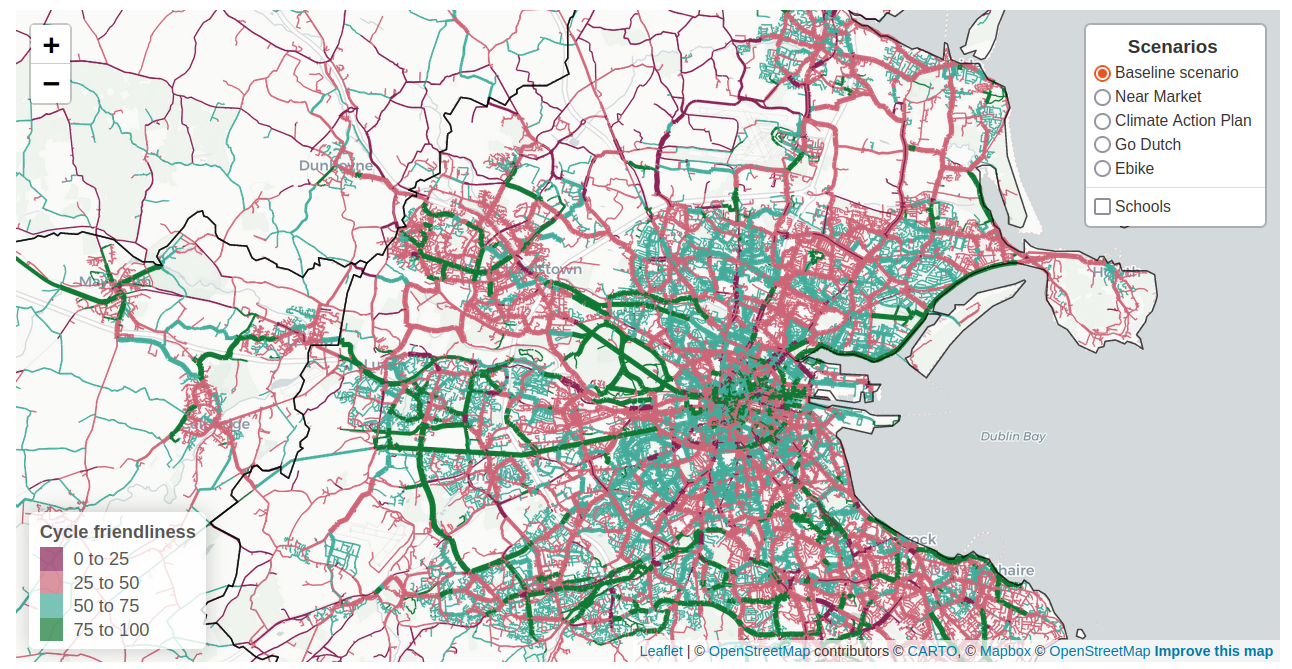
\includegraphics{images/paste-1.png}
%DIFDELCMD < 

%DIFDELCMD < 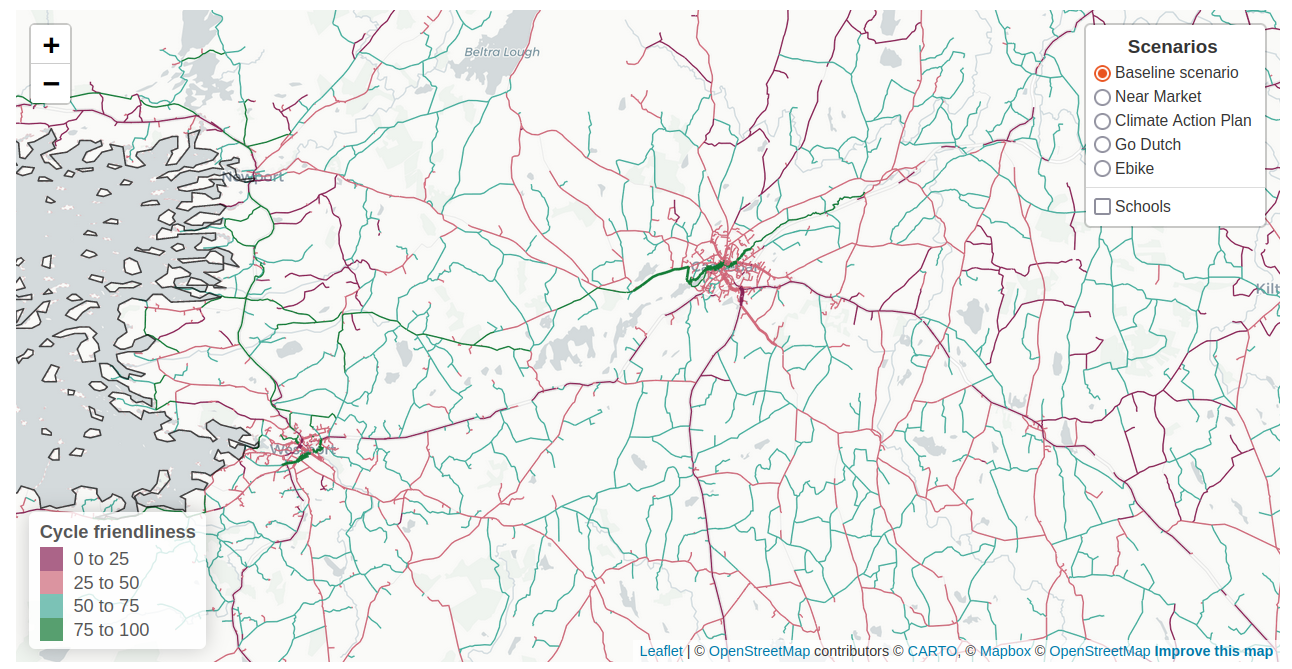
\includegraphics{images/paste-3.png}
%DIFDELCMD < 

%DIFDELCMD < }
%DIFDELCMD < %%%
\DIFdelendFL \DIFaddbeginFL \centering{

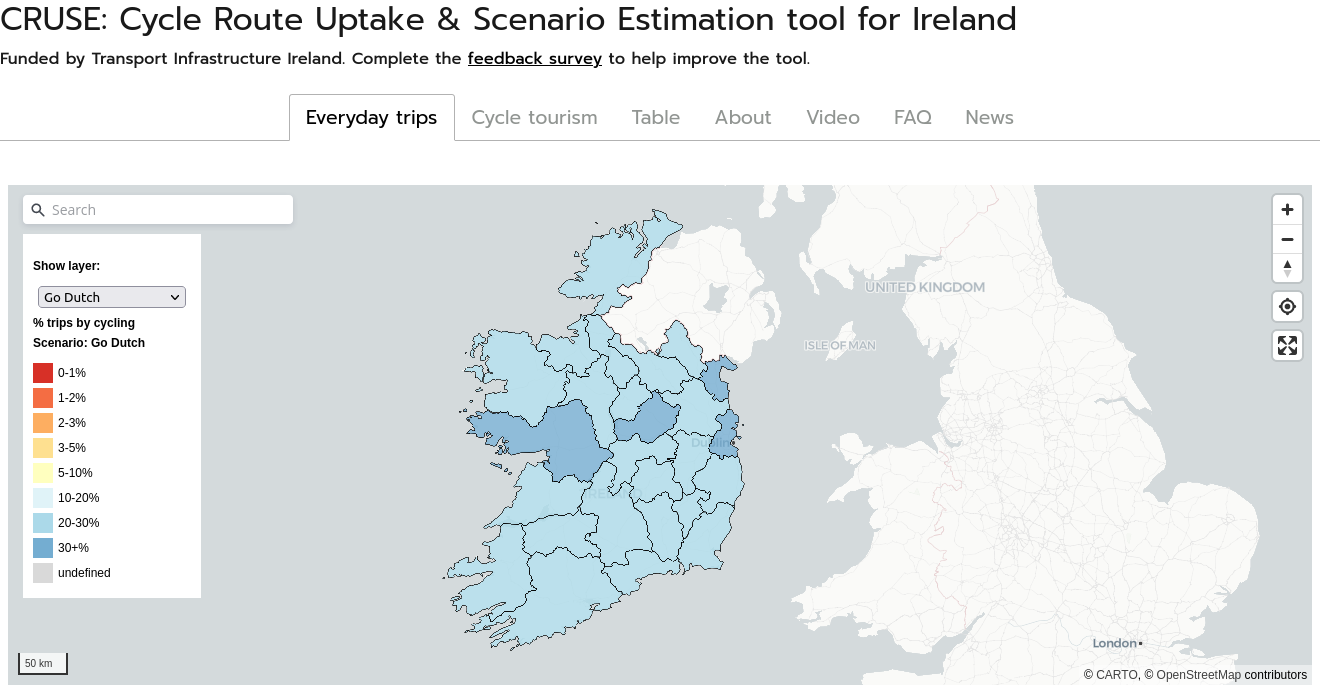
\includegraphics{images/paste-10.png}

}
\DIFaddendFL 

\caption{\DIFdelbeginFL %DIFDELCMD < \label{fig-dublin}%%%
\DIFdelendFL \DIFaddbeginFL \label{fig-landing}\DIFaddendFL Illustration of the \DIFdelbeginFL \DIFdelFL{density }\DIFdelendFL \DIFaddbeginFL \DIFaddFL{landing page }\DIFaddendFL of \DIFdelbeginFL \DIFdelFL{route networks
generated by }\DIFdelendFL the
CRUSE Tool for \DIFdelbeginFL \DIFdelFL{Dublin City and surroundings (top) and
rural County Mayo on the West coast of }\DIFdelendFL Ireland.\DIFdelbeginFL \DIFdelFL{Source: CRUSE Tool,
available at }%DIFDELCMD < \url{https://cruse.bike/}%%%
\DIFdelFL{.}\DIFdelendFL }

\end{figure}%

This paper \DIFdelbegin \DIFdel{aims to describe the design, features and potential use of }\DIFdelend \DIFaddbegin \DIFadd{describes an approach to strategic cycle network planning
tool development that is open, scalable, and evidence-based. We label
the approach Cycle Route Uptake and Scenario Estimation (CRUSE) and
present a case study of its application in Ireland, the results of which
are publicly available at }\href{https://cruse.bike/}{\DIFadd{cruse.bike}} \DIFadd{in }\DIFaddend the
CRUSE Tool \DIFaddbegin \DIFadd{for Ireland, the landing page of which is illustrated in
Figure~\ref{fig-landing}}\DIFaddend . In Section~\ref{sec-methods}, we outline the
methods used to generate the evidence presented in the CRUSE Tool. In
Section~\ref{sec-results}, we present the results of the CRUSE Tool,
including estimates of current cycling levels and future cycling
potential at the national, regional and local levels. In
Section~\ref{sec-discussion}, we discuss \DIFaddbegin \DIFadd{limitations and possible future
improvements to the approach, and }\DIFaddend the implications of the results for
\DIFdelbegin \DIFdel{policy and practice. In }\DIFdelend \DIFaddbegin \DIFadd{Ireland before making concluding remarks in
}\DIFaddend Section~\ref{sec-conclusions}\DIFdelbegin \DIFdel{, we conclude
the paper}\DIFdelend .

\section{\DIFdelbegin \DIFdel{Methods and data}\DIFdelend \DIFaddbegin \DIFadd{Tools for estimating cycling
potential}\DIFaddend }\DIFdelbegin %DIFDELCMD < \label{sec-methods}
%DIFDELCMD < %%%
\DIFdelend \DIFaddbegin \label{tools-for-estimating-cycling-potential}
\DIFaddend 

\DIFdelbegin \DIFdel{The methods used to generate the evidence presented in the CRUSE Tool
build on the Propensity to Cycle Tool (PCT) , which was originally funded
by the UK's Department for Transport and developed by a multi-university
team.
An important feature of the PCT is that it is open source and publicly available (at }\href{https://www.pct.bike/}{\DIFdel{www.pct.bike}}%DIFAUXCMD
\DIFdel{) }\DIFdelend \DIFaddbegin \DIFadd{Tools for estimating geographical distribution of cycling potential have
advanced substantially in recent years. Developed by researchers and
developers in academic, public and private sectors, they have evolved
from simple area-based static models tailored to specific regions to
more complex and (in some cases) more generalizable tools. These tools
can be considered as a specific application of the concept of planning
support systems (PSS) , which are designed to help planners and
decision-makers to make more informed decisions \mbox{%DIFAUXCMD
\citep{geertman2009}}\hspace{0pt}%DIFAUXCMD
.
Outputs include maps with results available at several levels of
analysis with levels of availability ranging from being only available
to researchers and in static maps to open access mapping systems
available to the public.
}

\DIFadd{Previous studies have applied the concept of PSS to specific modes,
including walking \mbox{%DIFAUXCMD
\citep{bencekri2024}}\hspace{0pt}%DIFAUXCMD
, public transport
\mbox{%DIFAUXCMD
\citep{barmentlo2012} }\hspace{0pt}%DIFAUXCMD
and cycling \mbox{%DIFAUXCMD
\citep{bencekri2023}}\hspace{0pt}%DIFAUXCMD
. While such prior
work provides insight into the potential for approaches to transport
planning that are both data-driven and participatory, the focus of this
paper is on tools that focus attention on the }\emph{\DIFadd{geographic
distribution}} \DIFadd{of cycling potential and which answer the question ``where
to build''. Not all papers reviewed in this section classify themselves
as, or even mention, PSS, but all of them can be considered as PSS. This
paper is informed by the thinking underlying PSS, including the idea
that the resulting tools are more effective if they are modular and can
inter-link with other tools and processes in the planning process: PSS
can be conceived as a ``toolbox with separate instruments that can work
and talk to each other effectively (as in the open systems concept) and
that will be selectively applied in varying configurations to support a
particular phase in the planning process'' \mbox{%DIFAUXCMD
\citep{geertman2002}}\hspace{0pt}%DIFAUXCMD
. We
share this conception of PSS, emphasizing the benefits of a focus on a
particular mode (cycling) and a particular phase in the planning process
(strategic network development).
}

\DIFadd{Some of the most relevant existing tools are summarised below and
presented in Table~\ref{tbl-tools}.
}

\begin{longtable}[t]{>{\raggedright\arraybackslash}p{13em}>{\raggedright\arraybackslash}p{15em}>{\raggedright\arraybackslash}p{12em}>{\raggedright\arraybackslash}p{5em}}

\caption{\label{tbl-tools}\DIFadd{Summary of existing tools for estimating
cycling potential.}}

\tabularnewline

\\
\toprule
\DIFadd{Approach }& \DIFadd{Coverage and input data }& \DIFadd{Outputs and availability }& \DIFadd{License}\\
\midrule
\cellcolor{gray!10}{Bicycle share model, Parkin et al. (2007)} & \cellcolor{gray!10}{England and Wales, Journeys to work OD census data, at the small-area (wards) level} & \cellcolor{gray!10}{Static tables in academic paper} & \cellcolor{gray!10}{Proprietary}\\
\DIFadd{Analysis of  Cycling Potential (ACP), Transport for London (2010}\DIFaddend , \DIFdelbegin \DIFdel{allowing its use by all stakeholders in the transport planning process
\mbox{%DIFAUXCMD
\citep{lovelace2017}}\hspace{0pt}%DIFAUXCMD
. The PCT approach has had major policy impacts, as
outlined in
Research Excellence Framework (REF) impact case studies,
which demonstrate that the tool ``revolutionized strategic cycle
planning in England and Wales'' by overcoming the barriers }\DIFdelend \DIFaddbegin \DIFadd{2016) }& \DIFadd{London, London Travel Demand Survey }& \DIFadd{Static tables, graphs, and heatmaps, not publicly available }& \DIFadd{Proprietary}\\
\cellcolor{gray!10}{Prioritization index, Larsen et al. (2013)} & \cellcolor{gray!10}{Montreal, Survey, Road safety, and OD data} & \cellcolor{gray!10}{Map-based heatmap, not publicly available} & \cellcolor{gray!10}{Proprietary}\\
\DIFadd{Usage intensity index, Zhang et al. (2014) }& \DIFadd{Belo Horizonte, Survey, census, and OD data }& \DIFadd{Static tables and maps, not publicly available }& \DIFadd{Proprietary}\\
\cellcolor{gray!10}{The Cycling Potential Tool (CPT), Phillips and Range (2017)} & \cellcolor{gray!10}{Scotland, Environmental and socioeconomic data, at the small area (output areas) level} & \cellcolor{gray!10}{Maps showing cycling potential in each area} & \cellcolor{gray!10}{Proprietary}\\
\addlinespace
\DIFadd{Propensity to Cycle Tool (PCT), Lovelace et al. (2017) }& \DIFadd{England and Wales, Journeys to work and school OD census data, at the small area (LSOA) level }& \DIFadd{Online maps, graphs, tables, publicly available at www.pct.bike }& \DIFadd{Open source}\\
\cellcolor{gray!10}{The    Gross Potential for Cycling tool (CPC), Silva et al. (2021 and 2022)} & \cellcolor{gray!10}{21 Portuguese cities, Land use and socio-demographic data, at the small area (census tract) level} & \cellcolor{gray!10}{Static maps showing cycling potential in different areas} & \cellcolor{gray!10}{NA}\\
\bottomrule

\end{longtable}

\DIFadd{Area-based approaches were developed before network-based tools, such as
a 2007 regression-based model to estimate the percentage of cycling
trips to work in England and Wales based on socioeconomic,
transportation, and physical factors at the small area (wards) level in
2007 \mbox{%DIFAUXCMD
\citep{parkin_estimation_2007}}\hspace{0pt}%DIFAUXCMD
. They found that areas with a higher
percentage of females, non-whites, car ownership, lower socioeconomic
classes, income, distance to work, population density, poor highway
conditions, hills, rainfall, and fewer off-road bicycle routes tended to
have a lower proportion of cycling to work. The approach also generated
``forecasts for potential levels of bicycle use'' with with increases in
off-road routes, improvements of highway and, conversely, increases in
car ownership and distance to work leading to decreases in cycling to
work.
}

\DIFadd{Three years later, Transport for London created the Analysis of Cycling
Potential (ACP) tool based on a mode choice model that assesses the
likelihood of trips being cycled, with data from the TfL London Travel
Demand Survey as its primary input. The tool generates tables, graphs,
and heatmaps showing the potential for cycling for different trips
purposes in London to guide local cycling initiatives, such as where new
hire `docking stations' should go. The tool does not use
origin-destination data and cannot estimate cycling potential on
specific routes \mbox{%DIFAUXCMD
\citep{transport_for_london_analysis_2010}}\hspace{0pt}%DIFAUXCMD
.
}

\DIFadd{Other tools that generate areal data to prioritize investment include a
study that generated a `prioritization index' for Montreal, Canada
\mbox{%DIFAUXCMD
\citep{larsen_build_2013}}\hspace{0pt}%DIFAUXCMD
, a `usage intensity index' based on stated
preferences in Belo Horizonte, Brazil, and a Cycling Potential Tool
(CPT) for Scotland \mbox{%DIFAUXCMD
\citep{phillips_development_2017}}\hspace{0pt}%DIFAUXCMD
. The CPT is
composed of the base environmental module --- based on eight weighted
factors (population density, hilliness, physical barriers, access to
services, existing cycling mode share, distance to work and school, and
road speed) --- and the quality of service module, which evaluates each
area of interest based on eight factors (surface condition, adjacent
cyclists, comfort factor, conflict, distance between junctions, slope,
access to services, and origin/destination).
}

\DIFadd{A more recent areal-based approach is the designed the Gross Potential
for Cycling (GPC) tool to prioritize areas for cycling infrastructure
and other cycling measures \mbox{%DIFAUXCMD
\citep{silva_gross_2021}}\hspace{0pt}%DIFAUXCMD
. The GPC uses two
sets of indicators: population-based indicators (age, potential demand
density, employment density and motorization rate) and area-based
indicators (accessibility, education, public transport, connectivity,
land use mix and relative performance). These indicators are calculated
considering topography, road hierarchy, and average congestion and
presented on a scale from 5 }\DIFaddend to \DIFdelbegin \DIFdel{cycling
investment imposed by lack of evidence on cycling
potential\mbox{%DIFAUXCMD
\citep{lovelace2023}}\hspace{0pt}%DIFAUXCMD
. }%DIFDELCMD < 

%DIFDELCMD < %%%
\DIFdel{The first version of
the PCT was based on }\DIFdelend \DIFaddbegin \DIFadd{10. They are then combined into an
overall score, weighted by their impact on cycling according to the
literature. The ranking of areas by the GPC are
}\href{https://boost.up.pt/en/ferramentas/gpc}{\DIFadd{publicly available}} \DIFadd{and
its practical value has been assessed through workshops
\mbox{%DIFAUXCMD
\citep{silva_revealing_2022}}\hspace{0pt}%DIFAUXCMD
.
}

\DIFadd{Route-based tools emerged with increasing availability of
origin-destination data, routing engines that can assign trips to
networks, and improvements in computer hardware and software needed to
generate route networks. A prominent example is the the Propensity to
Cycle Tool (PCT), first developed to estimate }\DIFaddend current and future \DIFdelbegin \DIFdel{potential
uptake of cycling for single stage }\emph{\DIFdel{travel to work}} %DIFAUXCMD
\DIFdelend \DIFaddbegin \DIFadd{levels
of cycling }\DIFaddend at desire line, zone, route, and route network levels \DIFdelbegin \DIFdel{\mbox{%DIFAUXCMD
\citep{lovelace2016}}\hspace{0pt}%DIFAUXCMD
. It was
launched in April }\DIFdelend \DIFaddbegin \DIFadd{for
case study cities \mbox{%DIFAUXCMD
\citep{lovelace_mapping_2016}}\hspace{0pt}%DIFAUXCMD
. The approach was
scaled-up to estimate estimate the potential benefits of uptake at zone
and desire line levels nationally, and launched as a publicly available
web application in }\DIFaddend 2017 \DIFdelbegin \DIFdel{as the government-endorsed tool for strategic
cycle network planning and part of the Cycling and Walking Investment
Strategy \mbox{%DIFAUXCMD
\citep{cycling2017}}\hspace{0pt}%DIFAUXCMD
}\DIFdelend \DIFaddbegin \DIFadd{\mbox{%DIFAUXCMD
\citet{lovelace2017}}\hspace{0pt}%DIFAUXCMD
}\DIFaddend . Extensions of the PCT
approach have included estimation of benefits at the individual level
\citep{woodcock2018}, addition of travel to school network
\citep{goodman2019}, and improved modeling of impacts on health,
environmental and distributional outcomes \citep{woodcock2021}.
Initially developed just for England, the PCT was extended to cover all
of Wales (for commuter data only) in 2018.

The PCT approach has been applied in other countries, including Ireland
(the topic of this paper), Scotland, and Portugal. In Portugal the
`biclaR' project, based on methods underlying the PCT, has been
developed and deployed for the Lisbon metro region. The resulting
evidence is available in an interactive web application hosted at
\href{https://biclar.tmlmobilidade.pt}{biclar.tmlmobilidade.pt}
\citep{felix2023}. biclaR includes estimates of impacts, using the World
Health Organisation (WHO) `HEAT for Cycling' tool and an `intermodality'
scenario that combines cycling with currently available public transit
options based on General Transit Feed Specification (GTFS) data.

The \DIFdelbegin \DIFdel{CRUSE Tool }\DIFdelend \DIFaddbegin \DIFadd{approach presented in this paper }\DIFaddend seeks to overcome \DIFdelbegin \DIFdel{the following methodological
limitations
of the original PCT: }%DIFDELCMD < 

%DIFDELCMD < \begin{itemize}
%DIFDELCMD < \tightlist
%DIFDELCMD < \item
%DIFDELCMD <   %%%
\DIFdel{Low }\DIFdelend \DIFaddbegin \DIFadd{three limitations
of previous tools to estimate cycling potential: 1) low }\DIFaddend resolution of
data, with routes starting and ending in administrative zone centroids\DIFdelbegin %DIFDELCMD < \item
%DIFDELCMD <   %%%
\DIFdel{Limited }\DIFdelend \DIFaddbegin \DIFadd{,
2) limited }\DIFaddend coverage of trip purposes beyond travel to work and school\DIFdelbegin %DIFDELCMD < \item
%DIFDELCMD <   %%%
\DIFdel{A }\DIFdelend \DIFaddbegin \DIFadd{,
and 3) a }\DIFaddend web interface that was not user-friendly or intuitive\DIFdelbegin %DIFDELCMD < \end{itemize}
%DIFDELCMD < 

%DIFDELCMD < %%%
\DIFdel{Methods were developed to overcome each of these, as outlined in
Section~\ref{sec-trip-purposes} to Section~\ref{sec-ui}}\DIFdelend .

\DIFaddbegin \section{\DIFadd{Methods and data}}\label{sec-methods}

\DIFaddend \subsection{Disaggregation of origin-destination
data}\label{sec-disaggregation}

A feature of active travel interventions is that they require dense
networks of routes to be effective \citep{parkin2018}. This means that
high levels of geographic resolution are needed in the data used to
estimate cycling potential. However, datasets on travel patterns are
often only available at the level of administrative zones. The Central
Statistics Office (CSO) in Ireland provides Place of Work, School or
College Census of Anonymized Records
(\href{https://www.cso.ie/en/census/census2016reports/powscar/}{POWSCAR})
data on the number of people traveling to work and school at the
Electoral Division (ED) level, for example.

In the PCT, the method used to convert OD data to route networks was to
calculate a single route between the population weighted centroids of
the zones associated with each OD pair. This method works fine when the
OD data represents movement between small areas, but was not appropriate
for generating route networks from the POWSCAR data because zone
centroids are so far apart that the resulting route networks would be
sparse and unrealistic. To tackle this issue we developed a new method
for OD data disaggregation called `jittering' \citep{lovelace2022}. The
method works by first disaggregating the OD data based on a
`disaggregation threshold' and then assigning each disaggregated
`sub-OD' pair to `subpoints' within each zone. As shown in
Figure~\ref{fig-dublin}, the resulting route networks are dense, even in
rural areas.

\DIFaddbegin \begin{figure}

\centering{

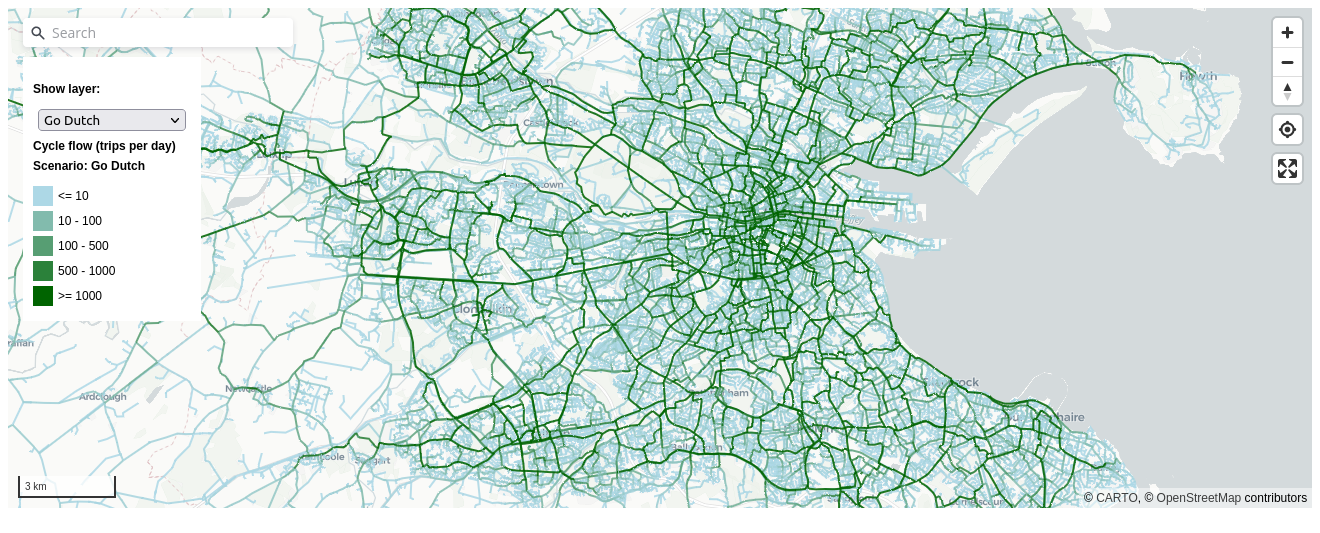
\includegraphics{images/paste-8.png}
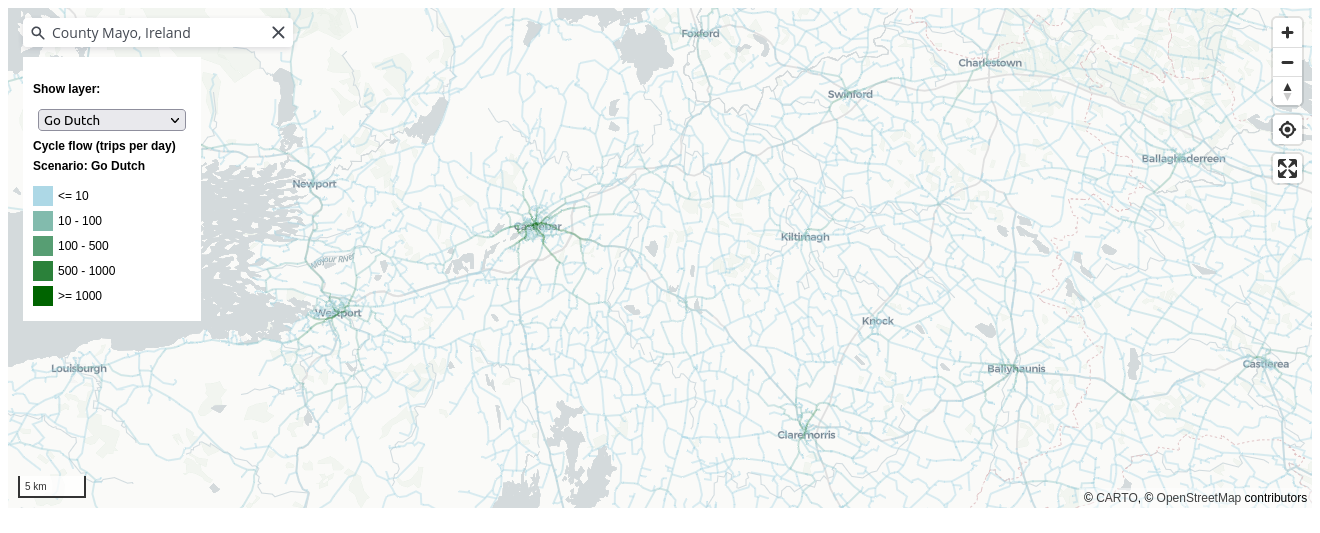
\includegraphics{images/paste-9.png}

}

\caption{\label{fig-dublin}\DIFaddFL{Illustration of the density of route networks
generated by the CRUSE Tool for Dublin City and surroundings (top) and
rural County Mayo on the West coast of Ireland (botton). Source: CRUSE
Tool, publicly available at }\href{https://cruse.bike/}{\DIFaddFL{cruse.bike}}\DIFaddFL{.}}

\end{figure}%DIF > 

\DIFaddend \subsection{Additional trip purposes}\label{sec-trip-purposes}

A limitation of the original PCT was that it only included travel to
work data. This was partially addressed by the inclusion of travel to
school based on data from the Department for Education in England
\citep{goodman2019}. An advantage of the POWSCAR OD data over OD
datasets derived from census surveys in many countries is that it
includes travel to school data. We commissioned a version of POWSCAR
that included a breakdown of the total flows between OD pairs by purpose
and mode, enabling a more realistic estimation of the `Baseline' cycling
network.

However, travel to school and work only constitute around only 30\% of
all trips in Ireland. To overcome this issue, we developed a spatial
interaction modeling methodology to estimate the number of trips between
each OD pair for additional trip purposes. The classification of trip
purposes used in the CRUSE Tool was guided mainly by the trip purpose
classification found within the National Household Travel Survey (NHTS),
but with the addition of categories based on the comprehensive POWSCAR
data, and the need to include recreational trips and multi-stage trips
(not yet implemented). An overview of the trip purposes used in CRUSE is
presented in Figure~\ref{fig-trip-purposes}.

\begin{figure}

\centering{

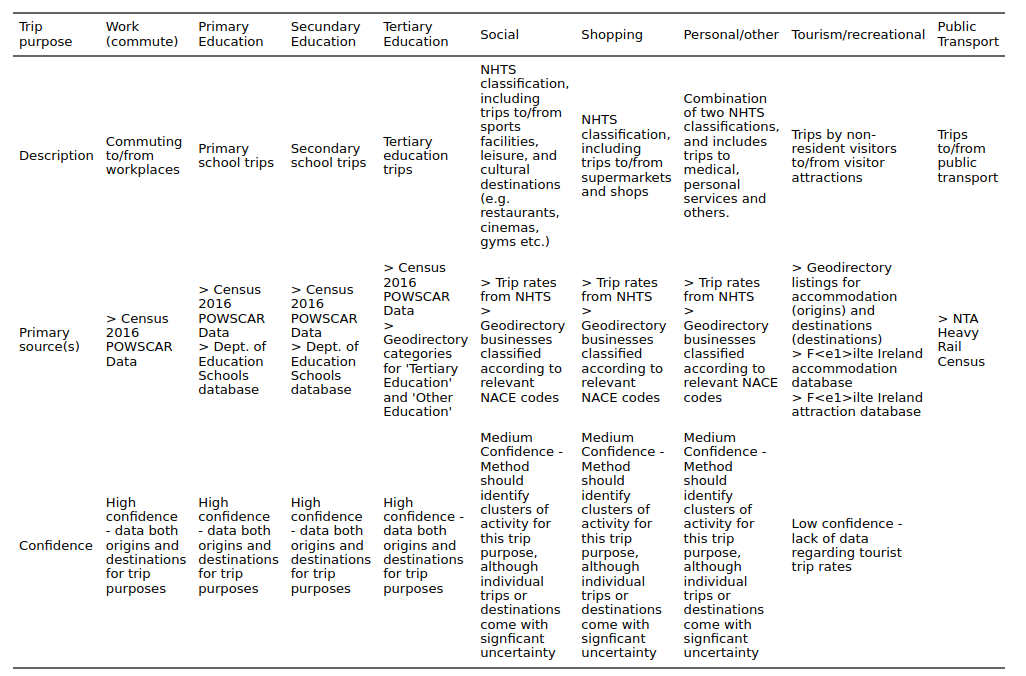
\includegraphics{images/paste-4.png}

}

\caption{\label{fig-trip-purposes}Trip purposes used in the CRUSE Tool.}

\end{figure}%

\subsection{Routing}\label{routing}

Routes in CRUSE are generated by CycleStreets, a not-for profit
transport consultancy and web development company who provide
application programming interfaces (APIs) supplying a range of datasets
for cycle planning and advocacy. Although based in Cambridge, UK,
CycleStreets provide routing services `by cyclists, for cyclists'
internationally, including in Ireland. The CycleStreets routing engine
is based on OpenStreetMap (OSM) data, which is continuously updated by a
global community of volunteers.

\DIFdelbegin \DIFdel{CycleStreets' services can be used by anyone for free , but }\DIFdelend \DIFaddbegin \DIFadd{While CycleStreets offers a free routing API, }\DIFaddend we commissioned a \DIFdelbegin \DIFdel{bespoke routing service for CRUSE, }\DIFdelend \DIFaddbegin \DIFadd{custom
routing service }\DIFaddend to enable:

\begin{itemize}
\tightlist
\item
  Calculation of hundreds-of-thousands of routes, which is beyond the
  terms of service of the free API.
\item
  Making changes to the routing profiles, including allowing routing on
  trunk roads, which are sometimes avoided in the default routing
  profiles.
\item
  Control over the version of OSM data being used for the routing,
  allowing regular updates to the route networks as OSM data is updated.
\end{itemize}

We calculated three network types for each disaggregated (`jittered') OD
pair: `Fastest', `Balanced' and `Quietest'. As outlined on the
CycleStreets'
\href{https://www.cyclestreets.net/help/journey/howitworks/}{website},
the `Fastest' routes minimize journey time, accounting for traffic
lights and surface type. The `Quietest' route type minimizes busy
sections of road, allowing high `diversion factors' from the fastest
route on quieter but less direct ways (often avoiding roads and
interactions with motor vehicles altogether where possible). The
`Balanced' route type is a compromize between the two, minimising
journey time while avoiding the busiest roads. Allowing users to switch
between these three route types enables them to consider the trade-offs
between directness and `cycle friendliness' when planning new
infrastructure, as shown in Figure~\ref{fig-route-types}.

These map are available on the `Route types' page for each county (see
\href{https://cruse.bike/kildare/route-types}{cruse.bike/kildare/route-types}).
In addition to showing the estimated routes under each scenario, the
page also presents summary statistics on the network:

\begin{itemize}
\item
  On the fastest network, 25\% of the distance cycled occurs in
  non-hostile segments and 7\% in cycle-friendly segments.
\item
  Under the baseline scenario, 52\% of the distance cycled on the
  quietest network occurs in non-hostile segments and 15\% in
  cycle-friendly segments.
\end{itemize}

These statistics can be revealing: in Kildare it suggests that around
half of all cycling activity occurs on network segments that are hostile
(with a high inferred level of traffic stress), even when efforts are
taken to avoid busy segments. For the Fastest network, which may be more
realistic for utility cycling, the proportion of cycling on hostile
segments is even higher at 75\%.

\begin{figure}

\begin{minipage}{0.50\linewidth}
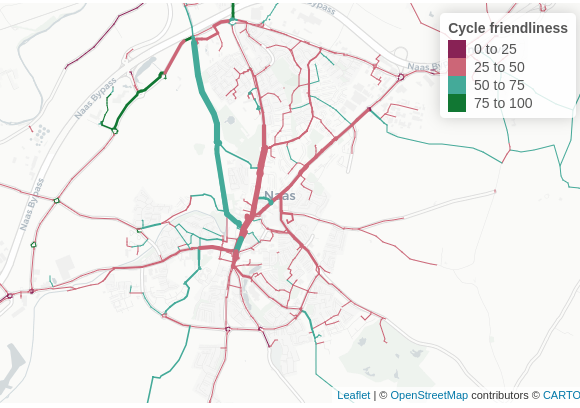
\includegraphics[width=2.60417in,height=\textheight]{images/naas_quietest_godutch.png}\end{minipage}%
%
\begin{minipage}{0.50\linewidth}
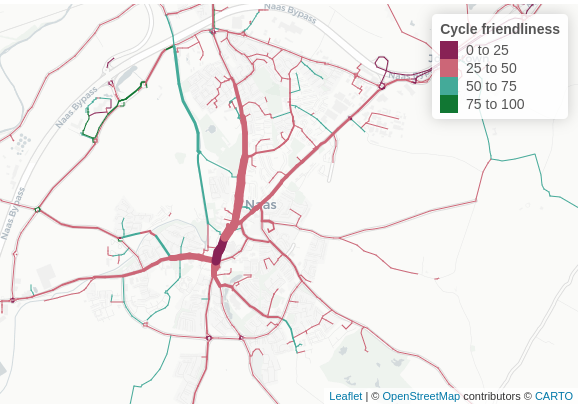
\includegraphics[width=2.60417in,height=\textheight]{images/naas_fastest_godutch.png}\end{minipage}%
\newline
\begin{minipage}{0.50\linewidth}
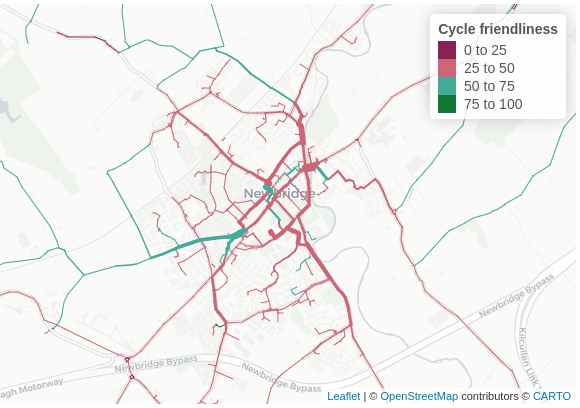
\includegraphics[width=2.60417in,height=\textheight]{images/newbridge_quietest_godutch.png}\end{minipage}%
%
\begin{minipage}{0.50\linewidth}
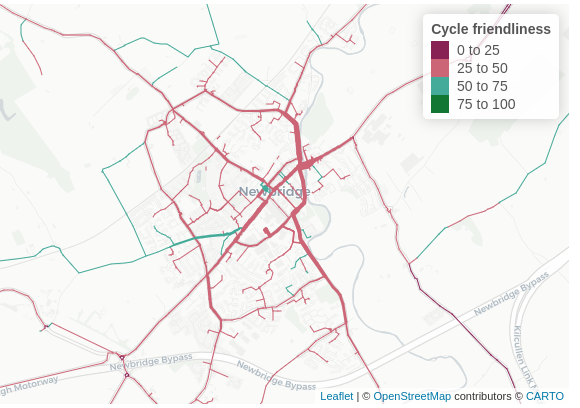
\includegraphics[width=2.60417in,height=\textheight]{images/newbridge_fastest_godutch.png}\end{minipage}%

\caption{\label{fig-route-types}Illustration of the Quietest (left) and
Fastest (right) route networks for Naas (top) and Newbridge (bottom).}

\end{figure}%

\subsection{Scenarios of cycling potential}\label{sec-scenarios}

The datasets outlined above were used to generate estimates of cycling
currently (the `Baseline' scenario) and under four scenarios of cycling
potential: Near Market, Climate Action Plan, Go Dutch, and Ebike. Each
of these scenarios is described below, as illustrated in
Figure~\ref{fig-scenarios}.

\begin{figure}

\centering{

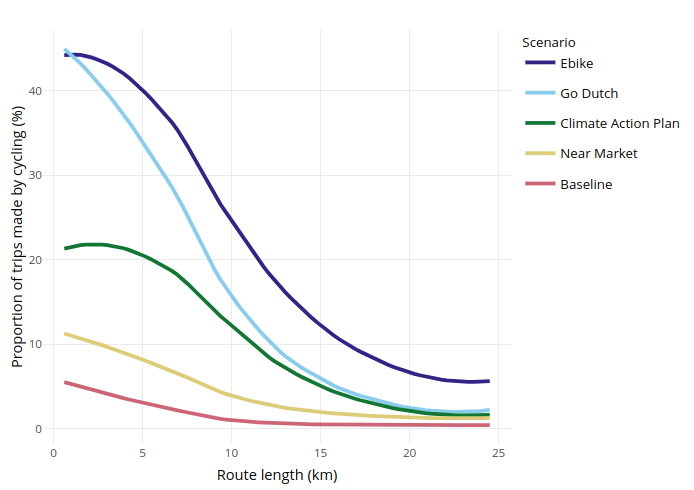
\includegraphics{images/scenarios_kildare.png}

}

\caption{\label{fig-scenarios}Distance-mode share graph for Kildare used
to communicate the different scenarios. Source: county level view for
Kildare in the open access CRUSE Tool at
\url{https://cruse.bike/kildare}.}

\end{figure}%

\subsubsection{Baseline}\label{baseline}

The Baseline scenario approximates current cycling levels. As outlined
in Section~\ref{sec-trip-purposes}, the Baseline scenario includes
travel to work and school, and additional trip purposes. Cycling levels
were taken from the POWSCAR data, which includes the number of people
traveling by each mode between each OD pair.

\subsubsection{Near Market}\label{near-market}

The Near Market scenario approximates the level of cycling that would be
achieved if levels of cycling uptake observed in areas of Ireland with
high levels of cycling according to the 2016 Census were achieved
everywhere, accounting for differences in trip distances and hilliness
levels. The scenario is implemented as follows:

\begin{itemize}
\tightlist
\item
  Calculate distance decay curves for Dublin for the base year (2016,
  using POWSCAR data) by fitting a model to the relevant OD data after
  it has been converted to a route network dataset
\item
  Apply the Near Market model to the hilliness and distance values for
  each county during the build process
\item
  Add the current level of cycling to the Near Market model
\end{itemize}

\subsubsection{Climate Action Plan}\label{climate-action-plan}

The Climate Action Plan scenario \DIFdelbegin \DIFdel{is loosely based on }\DIFdelend \DIFaddbegin \DIFadd{models the transport emissions
reductions targeted in }\DIFaddend the Irish Government's
\href{https://www.gov.ie/en/publication/6223e-climate-action-plan-2021/}{Climate
Action Plan 2021}, which \DIFdelbegin \DIFdel{contains policies for action to achieve }\DIFdelend \DIFaddbegin \DIFadd{aims for }\DIFaddend a 51\% \DIFdelbegin \DIFdel{reduction in overall GHG }\DIFdelend \DIFaddbegin \DIFadd{cut in overall greenhouse gas
}\DIFaddend emissions by 2030 \DIFdelbegin \DIFdel{, on a path towards }\DIFdelend \DIFaddbegin \DIFadd{as part of the pathway to }\DIFaddend net-zero \DIFaddbegin \DIFadd{emissions }\DIFaddend by 2050.
For transport, this includes 500,000 extra walking, cycling and public
transport trips per day by 2030. In terms of car travel, the target is
to ``Increas{[}e{]} the proportion of kilometers driven by passenger
electric cars to between 40 and 45\% by 2030, in addition to a reduction
of 10\% in kilometers driven by the remaining internal combustion engine
cars.'' This equates to a 5.5 to 6\% reduction in total car km driven.

To model this decrease in car driver km, cycling uptake increases in
line with the Go Dutch scenario. However, we only model shift from
driving to cycling. There is no shift from other modes of transport to
cycling.

\subsubsection{Go Dutch}\label{go-dutch}

Under the Go Dutch scenario cycling reaches levels equivalent to those
found in the Netherlands, taking account of the effects of route
hilliness (measured as mean gradient) and route distance. This scenario
uses the same model that was used PCT, allowing trips to shift from any
other mode to cycling \citep{lovelace2017}.

\subsubsection{Ebike}\label{ebike}

Also based on the PCT scenario with the same name, the Ebike scenario in
CRUSE takes Go Dutch cycling uptake, and adds onto this the impact of
increased ebike usage, which allows for longer cycle trips. However,
travel to primary and secondary schools still uses Go Dutch uptake,
since no ebike scenario has been developed for school journeys, and
children may be less likely to own ebikes than adults.

\subsection{User interface}\label{sec-ui}

The CRUSE web application is statically hosted, meaning that it can be
accessed without the need for a server running software such as the R
package `shiny' or Python packages such as `streamlit' or `flask' in the
background \citep{wickham2021}. Typical intended user stories are
illustrated in Figure~\ref{fig-user-stories}, which shows that the tool
is designed to be used by both professional and non-professional users.
For the main target audience, professional transport planners working at
the county level, the tool provides a range of outputs, including
estimates of cycling potential at the county and network level. The
provision of balanced (the default), quietest and fastest route networks
enables planners to consider the trade-offs between directness and
`cycle friendliness' when planning new infrastructure. The tool also
provides data downloads, enabling estimates of cycling potential on the
network to be visualised and analysed with other tools such as QGIS,
Python or R.

For non-professional users, the tool provides a simple interface to
explore the cycling potential of the network. By providing a single
landing page that is suitable for both professional and non-professional
users (such as an advocate or parent interested in safe routes to
school), the tool aims to facilitate communication between these groups.

\begin{figure}

\centering{

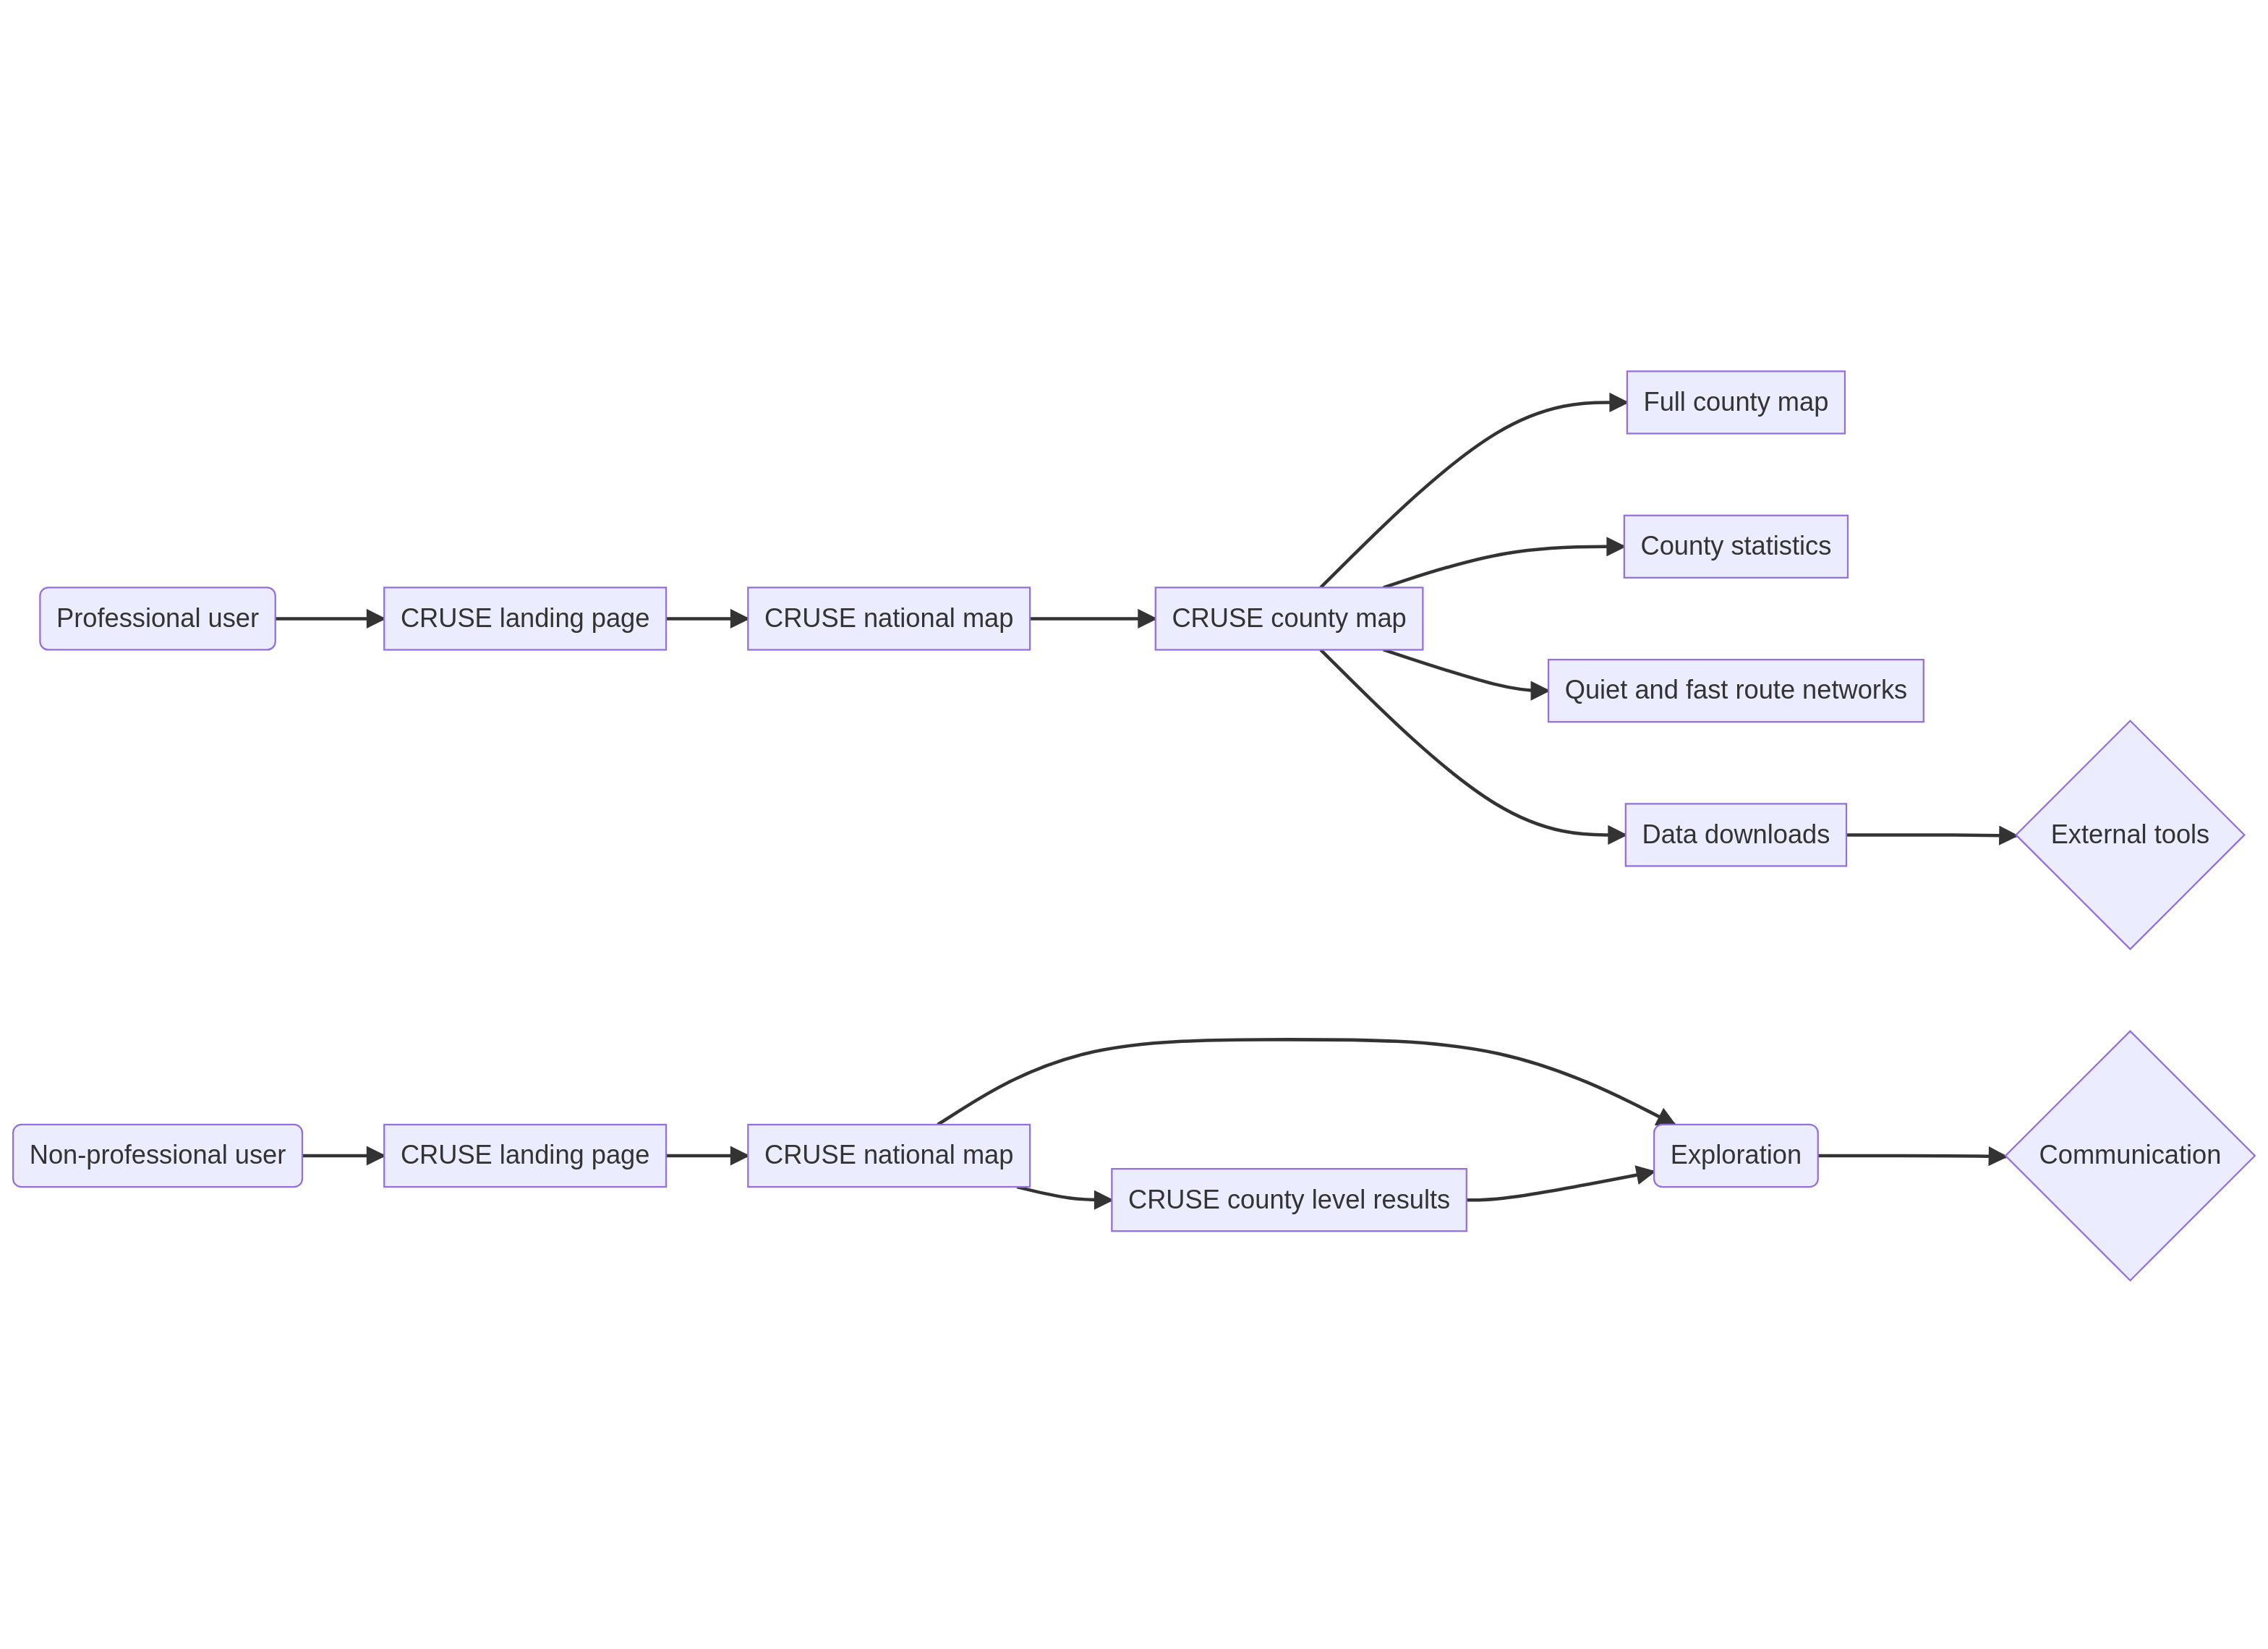
\includegraphics{images/mermaid-figure-1.png}

}

\caption{\label{fig-user-stories}Hypothetical user stories for the CRUSE
Tool illustrating that it can be used in different ways by different
user groups.}

\end{figure}%

\section{Results}\label{sec-results}

The main result of the work presented in this paper is an open access
web application and datasets on current and potential future cycling
levels in Ireland, with evidence provided at county and route segment
levels. Like \DIFdelbegin \DIFdel{the PCT on which CRUSE builds}\DIFdelend \DIFaddbegin \DIFadd{other national tools presented in Table~\ref{tbl-tools}}\DIFaddend , a
key feature of the results is that \DIFdelbegin \DIFdel{they are systematic and
available for all counties, and most
routes on which cycling is permitted, in Ireland.
The full set of results }\DIFdelend \DIFaddbegin \DIFadd{it provides a consistent and
objective baseline for comparing cycling potentials in different areas.
}

\DIFadd{The approach generates estimates of cycling potential on every road in
the country and }\DIFaddend are therefore too extensive to present in their entirety
in this paper. Through the interactive web application, users can
explore the data to generate the results that are most relevant to their
needs, whether that is finding the cycling potential on a particular
road or finding `weak links' or barriers in the cycle network associated
with a particular school, work place or other destination.

Instead of trying to show such use cases, of which there are many
hundreds, we present a selection of results to illustrate the main
features of the \DIFdelbegin \DIFdel{CRUSE Tool}\DIFdelend \DIFaddbegin \DIFadd{resulting evidence, in Section~\ref{sec-quantiative}. We
also present some qualitative results based on workshops and interviews
with stakeholders in Ireland, in Section~\ref{sec-qualitative}}\DIFaddend .

\DIFaddbegin \subsection{\DIFadd{Selected quantitative results}}\label{sec-quantiative}

\DIFaddend To illustrate the results in urban areas, we took the top 4 cities in
Ireland by population: Dublin City, Cork, Limerick and Galway (with city
populations of 0.6, 0.2, 0.1 and 0.1 million respectively). In
Figure~\ref{fig-city-results} we present the cycle route networks within
a 3km radius circle centred on each of these cities.

\begin{figure}

\centering{

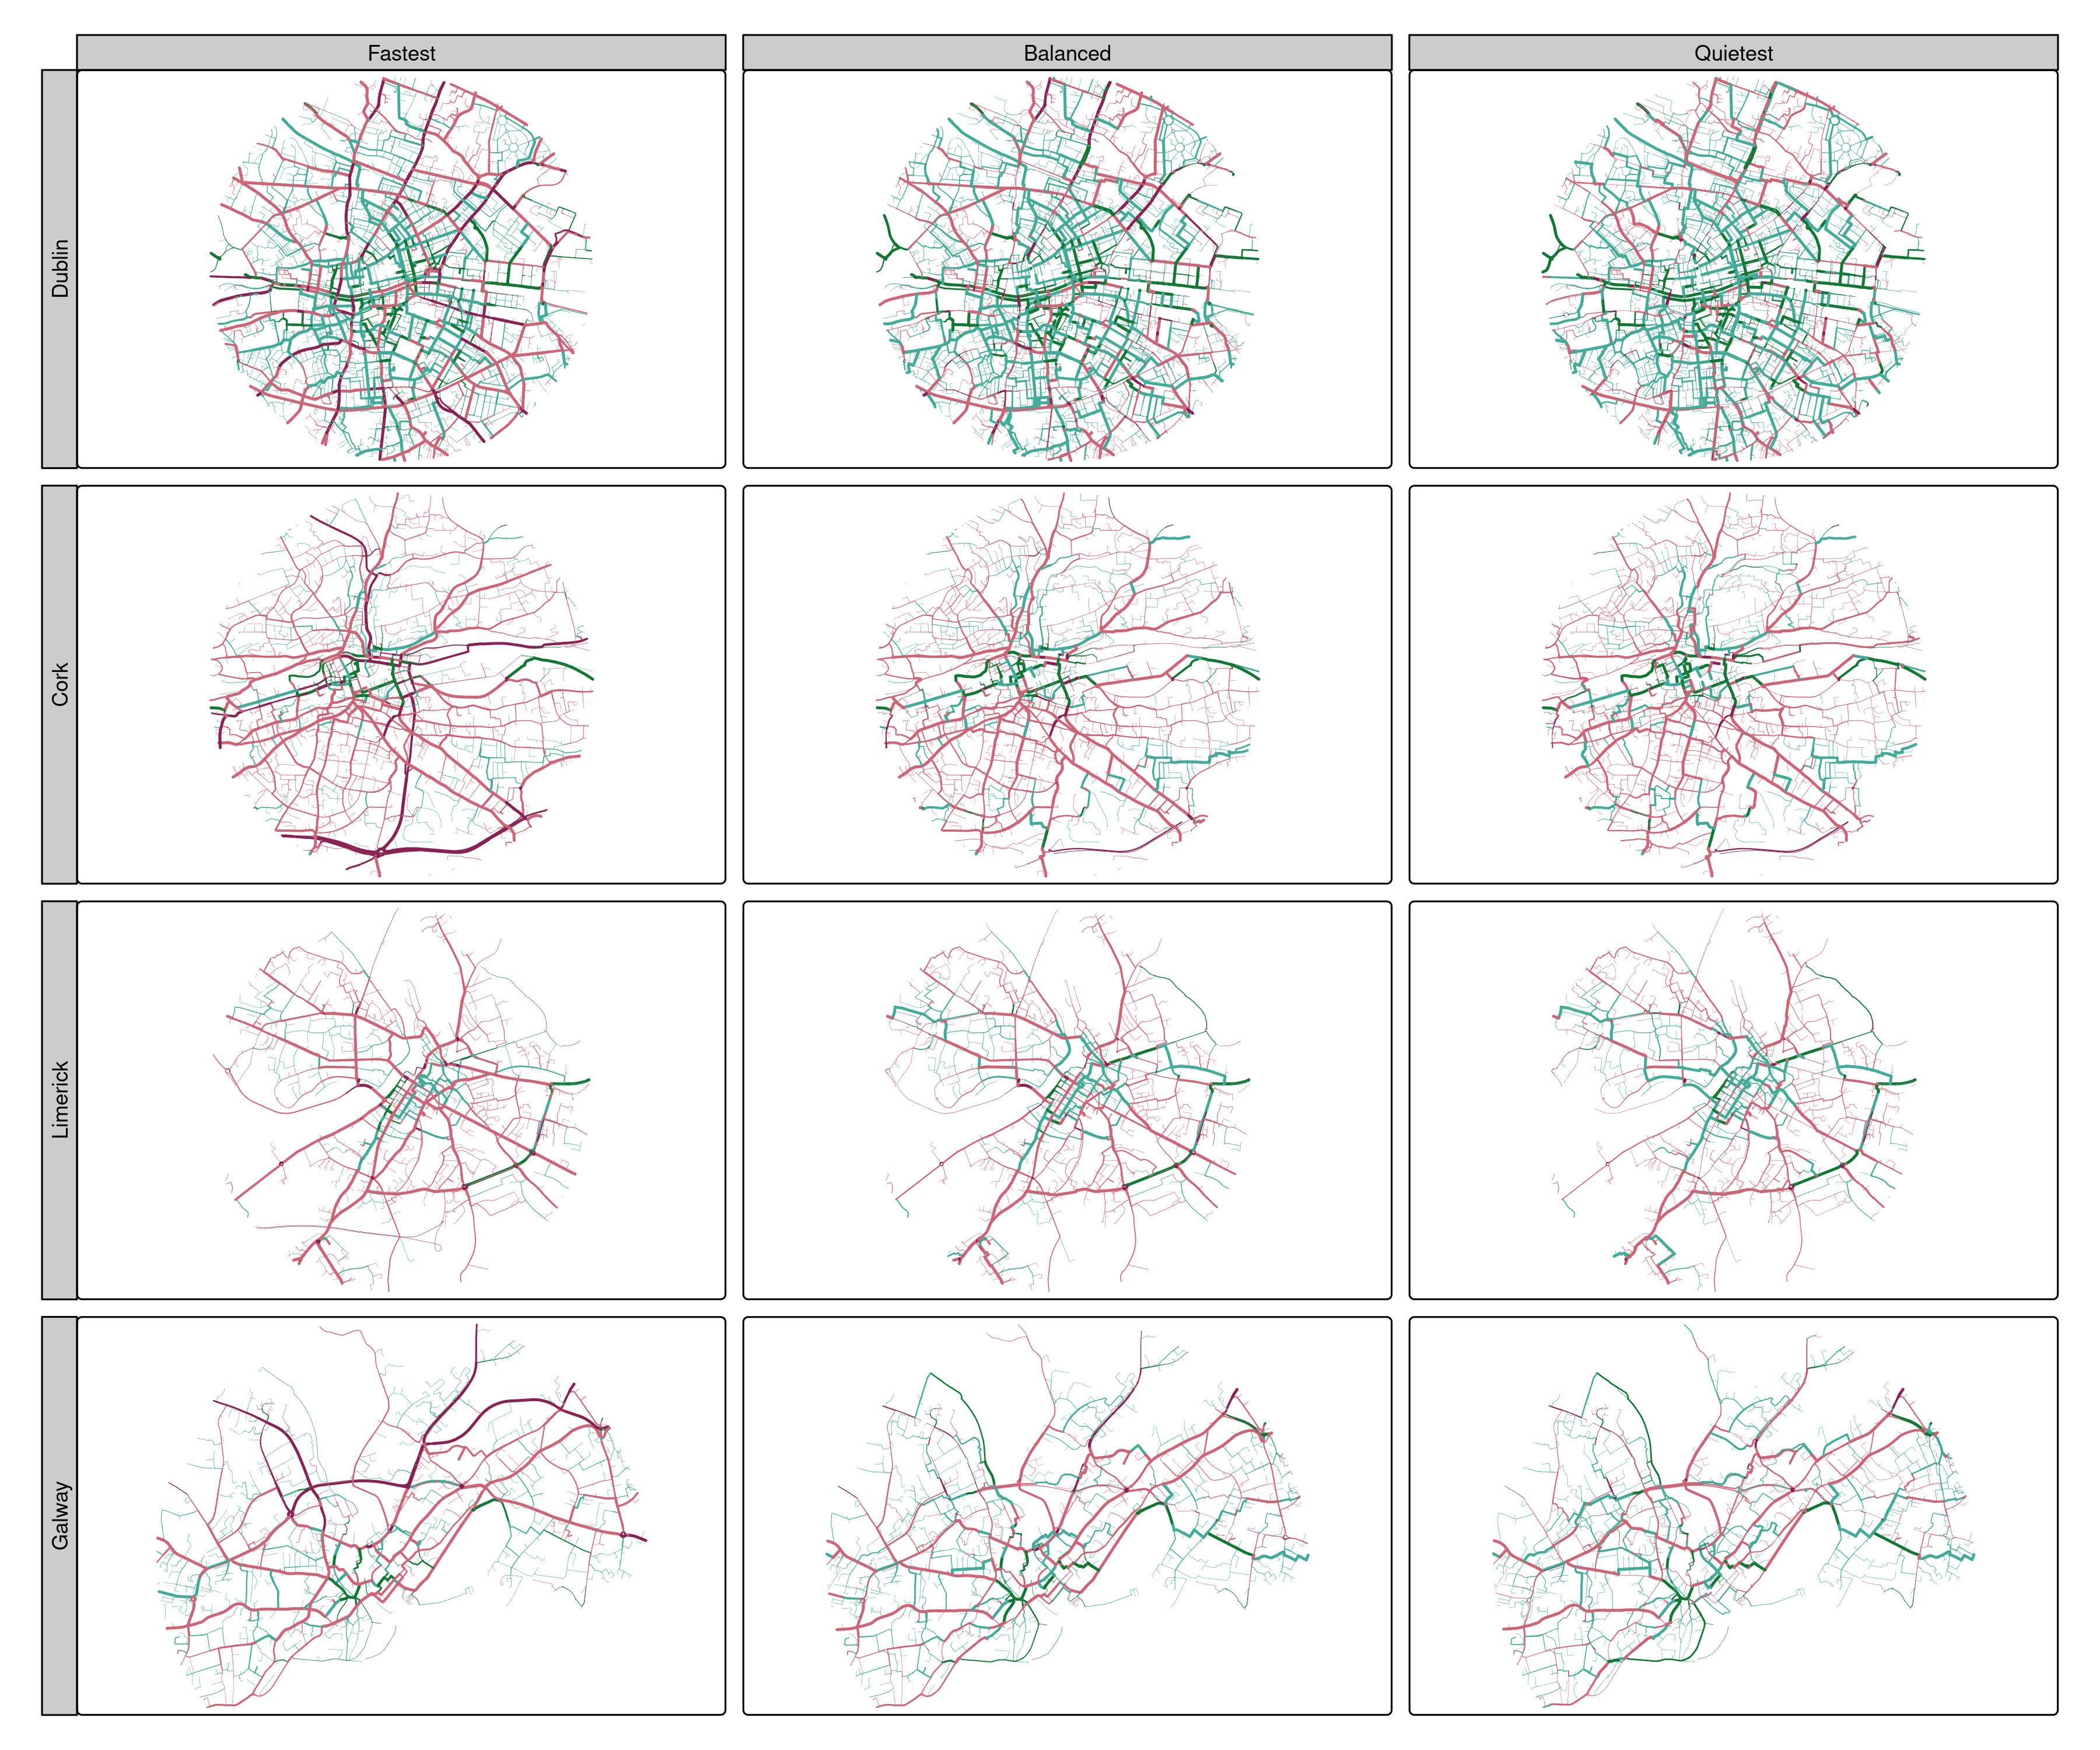
\includegraphics{images/rnet_types.png}

}

\caption{\label{fig-city-results}Fastest, balanced and quietest cycle
networks within 3km circular areas containing the four largest cities in
Ireland. The networks are coloured by cycle friendliness, with greener
segments representing more cycle friendly segments. Widths vary in
proportion to the potential level of cycling under the `Go Dutch'
scenario.}

\end{figure}%

Aside from the widely varying sizes and route networks of each city,
with Dublin having by far the densest network, it is clear from the
visualisation of cycling friendliness that there are many gaps in the
networks. Dublin has had received most investment in cycling
infrastructure and this is apparent from the high proportion of the
route network that is green, even in the `Fastest' route network
representing routes that prioritize speed and directness over comfort
and safety. Dublin also has the highest mode share of cycling of the
four cities, adding to the evidence base showing that investment in
cycling infrastructure is effective in increasing cycling uptake.

Although Dublin City has made progress, there are still many parts of
the Fastest route network, and even some parts of the Balanced and
Quietest route networks, that are not cycle friendly and which have high
cycling potential. According to a recent report, 71\% of residents in
the Dublin Metropolitan Area support ``more cycle tracks along roads,
physically separated from traffic and pedestrians'' \citep{walking2021}.
The results for the Dublin area could help prioritise investment in
cycling infrastructure in the city.

\DIFaddbegin \subsection{\DIFadd{Selected qualitative results}}\label{sec-qualitative}

\DIFadd{Thoughout the project, we undertook a series of workshops and interviews
with stakeholders in Ireland to gather feedback on the approach and
resulting tool. The feedback was generally positive, with stakeholders
commenting on the need for the tool, lack of data on cycling potential
proving a barrier to decision-making and investment, and the potential
for the tool. At an end of project workshop in December 2023,
stakeholders were asked to provide feedback on the tool and its
potential use in practice. Quotes and suggestions from these workshops,
and a subsequent interview with a Senior Transport Planning using the
evidence in their everyday work in Transport Infrastructure Ireland, and
presented in this section (with quotes being attributed to named
individuals where permission has been granted).
}

\DIFadd{Early in the project, we presented the approach to practitioners in
Kildare and Limmerick. The feedback from the workshop in Kildare
highlighted the need for the tool for practitioners at the county level,
as highlighted in the following quote:
}

\begin{quote}
\DIFadd{``It's a missing piece of evidence that will help new projects get
built'' (Senior Engineer, Sustainable Transport \& Traffic Management,
Kildare County Council)
}\end{quote}

\DIFadd{Practitioners in Kildare County Council that the evidence generated
}\emph{\DIFadd{was already valuable}} \DIFadd{the development of new cycle routes,
especially when making the case during planning applications. They
emphasized that cycle networks are often fragmented, and the tool allows
them to demonstrate how individual local schemes can contribute to a
larger, interconnected network. Council officers expressed a preference
for visualizations that directly compare the fast and quiet routes, as
they recognize the importance of both types of routes (users can switch
between the on the `Route types' page for each county although this
functionality is not available in the landing page map due to other
feedback requesting a simpler interface).
}

\DIFadd{In comparison with another tool (the National Transport Authority's
cycling propensity tool), the CRUSE tool was seen by practitioners in
Kildare as more user-friendly and intuitive, with the ability to
generate evidence at the route level, which is crucial for planning new
cycling infrastructure. Overall, the workshop participants concluded
that the approach filled gap in evidence and will greatly assist in the
development of new cycling projects.
}

\DIFadd{During the workshop with practitioners in Limerick, the estimates of
Baseline and Go Dutch potential at the network levels were found to
match well with local knowledge. The tool effectively highlighted the
same sections on the transport network that experienced planners
identified as priorities for investment in cycling, such as the South
Circular Road. Limerick County Council expressed their interest in
utilizing each network layer, particularly the quiet network, to support
new cyclists who lack confidence to share space with motor traffic.
Specific suggestions from the workshop included the suggestion to align
scenarios with national strategy (resulting in the Climate Action Plan
scenario) and to provide data downloads provided as `Shapefiles' for
further analysis (now implemented although the download format is
GeoPackage, an open standard for spatial data).
}

\DIFadd{In a subsequent interview with a practitioner using the evidence
generated by the CRUSE approach in their everyday work, we received the
following feedback. The outputs were a ``great tool for getting started
with project outline documents'' and ``ideal for generating a strategic
rationale for estimating demand and building the business case in the
absence of cycle count data'' (Declan Keenan, Senior Transport Planner
working on active travel, personal communication). Declan also noted the
alignment between local knowledge, cycle count data, and the outputs of
the approach: ``It's a good representation of what's going on'' and the
networks allign well in terms of network ``shape'' and the proportion of
trips of trips on different parts of the network. There were two
suggestions from Declan which have not yet been implemented: the
provision of data showing only ``gold standard'' POWSCAR data, and the
need for training on the tool to ensure that all staff can use it
effectively. These, and other potential improvements, are discussed in
the next section.
}

\DIFaddend \section{Discussion}\label{sec-discussion}

The aim of the paper was to describe the design, features and potential
use of the \DIFdelbegin \DIFdel{CRUSE Tool}\DIFdelend \DIFaddbegin \DIFadd{`CRUSE' approach and resulting tool}\DIFaddend . As outlined in the
previous section, the CRUSE Tool provides evidence on current and
potential future cycling levels across Ireland down to the street level,
with potential assigned to `fastest', `balanced' and `quietest' route
networks. This provision of multiple scenarios of behavior change
\emph{and} multiple scenarios of investment, for example in cycling
infrastructure next to major roads vs quiet residential streets, is a
key feature of the CRUSE Tool.

\DIFaddbegin \subsection{\DIFadd{Uses of the tool in
practice}}\label{uses-of-the-tool-in-practice}

\DIFaddend As highlighted in a paper on cycling infrastructure preferences based on
a case study of Dublin, both directness and quietness are important
\citep{caulfield2012}:

\begin{quote}
Direct routes with short journey times were found to be the most
important positive variable for existing cyclists and non-cyclists in
determining route choice. This is followed by infrastructure type, the
number of junctions along the route, traffic speed and cyclist volumes.
In terms \DIFdelbegin \DIFdel{if }\DIFdelend \DIFaddbegin \DIFadd{of }\DIFaddend infrastructure, regardless of the level of cycling
confidence, routes which have `no facilities' or `bus/cycle lanes' are
the least favoured cycle route types.
\end{quote}

The CRUSE Tool can help both in terms of describing the current
situation, and also prioritise investment in those direct routes with
high cycling potential that lack adequate cycling infrastructure
\citep{caulfield2012}. It will also support reporting for the RISM
Directive on road casualties as part of the road safety management
system.

\DIFaddbegin \subsection{\DIFadd{Comparison with other tools and contribution to the
field}}\label{comparison-with-other-tools-and-contribution-to-the-field}

\DIFaddend While the CRUSE Tool is not the first national and publicly available
tool for cycling planning, it has some key features that make it
relevant for other countries, regions and road authorities tasked with
making their transport systems safe and sustainable:

\begin{itemize}
\tightlist
\item
  The results are \emph{open access} meaning that any stakeholder in the
  planning system can access the evidence. This will help to democratize
  the transport planning process and make wider conversations about
  transport planning more evidence-based and less polarized
  \citep{lovelace2020}, something that is particularly relevant given
  the potentially polarizing nature of pro-cycling interventions
  \citep{wild2017}.
\item
  The results are fully reproducible (code to be released pending
  sign-off by TII's IT team), preventing `cloud lock in' to a
  potentially monopolistic consultancy, and encouraging input from the
  wider open source community \citep{lovelace2021, dhir2017}.
\item
  By covering a wide range of trip purposes --- not just travel to work
  \citep{lovelace2017, heinen2010} and travel \DIFaddbegin \DIFadd{to }\DIFaddend school
  \citep{goodman2019} as covered in previously published research on
  open access national cycle network planning tools --- the results
  capture a higher proportion of cycling potential including key rural
  trips which are often under-represented in models of active travel.
\end{itemize}

As the benefits of strategic planning for cycling become more apparent
\citep{scappini2022} we expect the demand for tools such as CRUSE to
grow. \DIFaddbegin \DIFadd{However, the approach is not without limitations and does not meet
all requirements in Ireland or indeed any country where the methods are
applied.
}

\DIFadd{A limitation of the approach as implemented in the CRUSE tool is that
the results are `static', reducing its ability to support monitoring of
growth in cycling, upgrades of existing cycling infrastructure and
dynamic (year-by-year) exposure information to estimate crash rates.
Exposure information is a key part of the the European RISM Directive,
for reporting collision rates of vulnerable road users by 2024. These
factors mean that the tool can be seen as an open access `leverage
point', providing key information for and supporting ambitious plans in
many aspects the planning system, from network design to post-build
monitoring \mbox{%DIFAUXCMD
\citep{lovelace2020}}\hspace{0pt}%DIFAUXCMD
.
}\DIFaddend 

\section{Conclusions}\label{sec-conclusions}

The CRUSE Tool is an open access web application for strategic cycle
network planning and prioritization of road safety interventions across
Ireland. Building on previous work, it provides a nationally consistent
evidence base, providing valuable insights to planners and other
stakeholders in the transport planning process, at national and local
levels. Because the results are available at the route segment level,
the tool can be used to identify `weak links' in the cycle network
\citep{vybornova2022}, and to prioritize investment in cycling
infrastructure to maximize health, equality, and other benefits
\citep{mahfouz, woodcock2021}. Furthermore, the provision of the
evidence in a free and publicly available website, hosted at
\href{https://cruse.bike}{cruse.bike}, means that it can be used by
anyone, encouraging wider participation and more evidence-based debate
about transport planning.

A key feature of the project methodologically is its calculation of
current and future potential not only for travel to work and travel to
school, but also for other trip purposes, including recreational trips.
This required the development of spatial interaction models and
estimation of the relative attractiveness of different destinations for
different trip purposes, an area of active research where new
developments could be incorporated into the tool in future
\citep{hasova2022}.

The CRUSE Tool and the underlying research and methods are not without
limitations, suggesting future areas of research, data collection needs,
and policy application. The route network level results have not been
validated to the extent we had planned at the outset of the project. We
compared route network level results with `ground truth' data from cycle
counter datasets across Dublin to test different network types and to
ensure that additional trip types added to work and educational trips
increased the quality of fit under the baseline scenario. However, the
size of the counter network was insufficient to provide an opportunity
for robust evaluation of model performance, suggesting a combined
program of new count data collection and analysis should be a priority
for future work, with findings feeding directly into work to improve the
outputs of the the CRUSE Tool.

More broadly, the tool's outputs are limited to just one mode of active
travel (cycling), ignoring walking and wheeling, including wheelchair
use and a range of wheeled devices such as scooters, bike trailers and
e-cargo bikes that can be used to escort children to school. Sustainable
transport policies should plan for walking, wheeling and cycling, and
there are many co-benefits of broadly defined active travel
interventions that benefit all active modes, such as measures to reduce
heavy motor traffic speeds and volumes in areas and along corridors with
high active travel potential. This raises the question of whether other
active modes should be incorporated into the results using the OD-based
approach outlined in this paper, or whether different modeling
approaches are needed to properly capture the shorter distance trips
typically made by walking \citep{cooper2018}. Furthermore, the estimates
of cycling presented in the CRUSE Tool omit multi-modal trips including
public transport, and omit trip chaining, due to the need to capture a
large portion of cycling potential within the resource constraints of
the project.

The CRUSE Tool is already used in practice to support more ambitious and
data-driven planning for safe cycling routes in multiple counties across
Ireland. We hope that the underlying approach, and the publicly
available evidence provided in the CRUSE Tool itself, provide a basis
for future reproducible research, open source software development into
strategic cycle network planning tools in Ireland and other countries.
Active travel represents a win-win-win for physical activity,
environment, and local economic opportunities. In combination with
broader sustainable mobility measures and policies to reduce motor
traffic speeds and volumes, tools such as CRUSE can support the fast and
fair decarbonisation of transport systems worldwide.

\section{List of abbreviations}\label{list-of-abbreviations}

APIs: Application Programming Interfaces

CSO: Central Statistics Office

CRUSE: Cycle Route Uptake and Scenario Estimation

ED: Electoral Division

GHG: Greehouse Gas

GTFS: General Transit Feed Specification

KSI: Killed and Seriously Injured

NRA: National Road Authority

NRN: National Road Network

OD: Origin-Destination, typically referring to origin-destination data
which contains information on the number of people traveling between
each pair of zones

OSM: Open Street Map

PCT: Propensity to Cycle Tool

POWSCAR: Place of Work, School or College Census of Anonymized Records

TII: Transport Infrastructure Ireland

\section{Declarations}\label{declarations}

\subsection*{Availability of data and
material}\label{availability-of-data-and-material}
\addcontentsline{toc}{subsection}{Availability of data and material}

Data was obtained from the Central Statistics Office (CSO) and Transport
Infrastructure Ireland (TII) under license and cannot be shared
publicly. The code used to generate the results presented in this paper
is fully reproducible and available at {[}to be added post review.{]}

\subsection*{Funding}\label{funding}
\addcontentsline{toc}{subsection}{Funding}

This work was funded by Transport Infrastructure Ireland (TII).

\subsection*{Acknowledgements}\label{acknowledgements}
\addcontentsline{toc}{subsection}{Acknowledgements}

{[}To be added post review.{]}


  \DIFdelbegin %DIFDELCMD < \bibliography{bibliography.bib}
%DIFDELCMD < %%%
\DIFdelend \DIFaddbegin \bibliography{bibliography.bib,cruse.bib,references.bib}
\DIFaddend 


\end{document}
